\Chapter{Combat}
{Looking back now, I wonder what I was thinking. I knew that elves rarely trusted outsiders, and threatening them with exposure was foolish.

The elven trader responded to my threat by swinging a dagger at my neck. Her first swipe was so fast I barely saw it; the sharp blade cut a deep score in my left shoulder. We scuffled briefly, but in the close confines of the trading room she could not use her greater speed to advantage, and I was much stronger. I was forced to kill her, although she wounded me more than once before our struggle ended.}{Esreva's Journal}

\Capitalize{W}{hether} in a gladiatorial arena, a battlefield in the middle of city-state wars, or surviving in the wasteland, adventurers in {\tableheader Dark Sun} find themselves entangled in combat situations. This chapter provides the rules to solve those combat situations.

\section{How Combat Works}
Combat is cyclical; everybody acts in turn in a regular cycle of rounds. Combat follows this sequence:

\begin{enumerate*}
\item Each combatant starts out flat-footed. Once a combatant acts, he or she is no longer flat-footed.

\item Determine which characters are aware of their opponents at the start of the battle. If some but not all of the combatants are aware of their opponents, a surprise round happens before regular rounds of combat begin. The combatants who are aware of the opponents can act in the surprise round, so they roll for initiative. In initiative order (highest to lowest), combatants who started the battle aware of their opponents each take one action (either a standard action or a move action) during the surprise round. Combatants who were unaware do not get to act in the surprise round. If no one or everyone starts the battle aware, there is no surprise round.

\item Combatants who have not yet rolled initiative do so. All combatants are now ready to begin their first regular round of combat.

\item Combatants act in initiative order (highest to lowest).

\item When everyone has had a turn, the combatant with the highest initiative acts again, and steps 4 and 5 repeat until combat ends.
\end{enumerate*}

\section{Combat Statistics}
This section summarizes the statistics that determine success in combat, and then details how to use them.

\subsection{Attack Roll}
An attack roll represents your attempt to strike your opponent on your turn in a round. When you make an attack roll, you roll:

\begin{Formula*}{1d20 + \textit{attack bonus}}
	\item \textit{Melee attack bonus} = base attack bonus + Str. modifier
	\item \textit{Ranged attack bonus} = base attack bonus + Dex. modifier + size modifier + range penalty.
\end{Formula*}

Other modifiers may also apply to this roll. If your result equals or beats the target's Armor Class, you hit and deal damage.

\textbf{Automatic Misses and Hits:} A natural 1 (the d20 comes up 1) on an attack roll is always a miss. A natural 20 (the d20 comes up 20) is always a hit. A natural 20 is also a threat---a possible critical hit.

\textbf{Base Attack Bonus:} A base attack bonus is an attack roll bonus derived from character class and level or creature type and Hit Dice (or combinations thereof). Base attack bonuses increase at different rates for different character classes and creature types. A second attack is gained when a base attack bonus reaches +6, a third with a base attack bonus of +11 or higher, and a fourth with a base attack bonus of +16 or higher. Base attack bonuses gained from different sources, such as when a character is a multiclass character, stack.

\textbf{Size Modifier:} This modifier captures the difference in size between creatures. If the creatures are of the same size, they strike each other normally, since the same size modifier applies to Armor Class.

\Table{Size Modifier}{p{1cm}XCp{1cm}}{
& \tableheader Size & \tableheader Size Modifier &\\
& Colossal & $-8$ &\\
& Gargantuan & $-4$ &\\
& Huge & $-2$ &\\
& Large & $-1$ &\\
& Medium & +0 &\\
& Small & +1 &\\
& Tiny & +2 &\\
& Diminutive & +4 &\\
& Fine & +8 &\\
}

\textbf{Range Penalty:} All ranged weapons have a range increment. Any attack from a distance of less than one range increment is not penalized for range. However, each full range increment imposes a cumulative $-2$ penalty on the attack roll. A thrown weapon has a maximum range of five range increments. A projectile weapon can shoot out to ten range increments.

\Figure*[\textwidth-5mm]{t}{images/battle-2.png}
\subsection{Damage}
When your attack succeeds, you deal damage. The type of weapon used determines the amount of damage you deal. Effects that modify weapon damage apply to unarmed strikes and the natural physical attack forms of creatures.

Damage reduces a target's current hit points.

\textbf{Minimum Damage:} If penalties reduce the damage result to less than 1, a hit still deals 1 point of damage.

\textbf{Strength Bonus:} When you hit with a melee or thrown weapon, including a sling, add your Strength modifier to the damage result. A Strength penalty, but not a bonus, applies on attacks made with a bow that is not a composite bow.

\textit{Off-Hand Weapon:} When you deal damage with a weapon in your off hand, you add only \onehalf your Strength bonus.

\textit{Wielding a Weapon Two-Handed:} When you deal damage with a weapon that you are wielding two-handed, you add 1\onehalf times your Strength bonus. However, you don't get this higher Strength bonus when using a light weapon with two hands.

\textbf{Multiplying Damage:} Sometimes you multiply damage by some factor, such as on a critical hit. Roll the damage (with all modifiers) multiple times and total the results. \textit{Note:} When you multiply damage more than once, each multiplier works off the original, unmultiplied damage.

\textit{Exception:} Extra damage dice over and above a weapon's normal damage are never multiplied.

\textbf{Ability Damage:} Certain creatures and magical effects can cause temporary ability damage (a reduction to an ability score).
\subsection{Armor Class}
Your Armor Class (AC) represents how hard it is for opponents to land a solid, damaging blow on you. It's the attack roll result that an opponent needs to achieve to hit you. Your AC is equal to the following:

{
	\centering
	\vskip1em
	{\Large 10 + \textit{armor bonus} + \textit{shield bonus}\\+ \textit{Dex. modifier} + \textit{size modifier}}
	\vskip1em
}

Note that armor limits your Dexterity bonus, so if you're wearing armor, you might not be able to apply your whole Dexterity bonus to your AC.

Sometimes you can't use your Dexterity bonus (if you have one). If you can't react to a blow, you can't use your Dexterity bonus to AC. (If you don't have a Dexterity bonus, nothing happens.)

\textbf{Other Modifiers:} Many other factors modify your AC.

\textit{Enhancement Bonuses:} Enhancement effects make your armor better.

\textit{Deflection Bonus:} Magical deflection effects ward off attacks and improve your AC.

\textit{Natural Armor:} Natural armor improves your AC.

\textit{Dodge Bonuses:} Some other AC bonuses represent actively avoiding blows. These bonuses are called dodge bonuses. Any situation that denies you your Dexterity bonus also denies you dodge bonuses. (Wearing armor, however, does not limit these bonuses the way it limits a Dexterity bonus to AC.) Unlike most sorts of bonuses, dodge bonuses stack with each other.

\textbf{Touch Attacks:} Some attacks disregard armor, including shields and natural armor. In these cases, the attacker makes a touch attack roll (either ranged or melee). When you are the target of a touch attack, your AC doesn't include any armor bonus, shield bonus, or natural armor bonus. All other modifiers, such as your size modifier, Dexterity modifier, and deflection bonus (if any) apply normally.

\subsection{Hit Points}
When your hit point total reaches 0, you're disabled. When it reaches $-1$, you're dying. When it gets to $-10$, you're dead.

\subsection{Speed}
Your speed tells you how far you can move in a round and still do something, such as attack or cast a spell. Your speed depends mostly on your race and what armor you're wearing.

Aarakocras, dwarves, and halflings have a speed of 6 meters (4 squares), or 4.5 meters (3 squares) when wearing medium or heavy armor (except for dwarves, who move 6 meters in any armor).

Humans, half-elves, muls, and pterrans have a speed of 9 meters (6 squares), or 6 meters (4 squares) in medium or heavy armor.

Elves, half-giants, and thri-kreen have a speed of 12 meters (8 squares), or 9 meters (6 squares) in medium or heavy armor.

If you use two move actions in a round (sometimes called a ``double move'' action), you can move up to double your speed. If you spend the entire round to run all out, you can move up to quadruple your speed (or triple if you are in heavy armor).
\subsection{Saving Throws}
Generally, when you are subject to an unusual or magical attack, you get a saving throw to avoid or reduce the effect. Like an attack roll, a saving throw is a d20 roll plus a bonus based on your class, level, and an ability score. Your saving throw modifier is:

{
	\centering
	\vskip1em
	\Large \textit{Base save bonus} + \textit{ability modifier}
	\vskip1em
}

\textbf{Base Save Bonus:} A saving throw modifier derived from character class and level. Base save bonuses increase at different rates for different character classes. Base save bonuses gained from different classes, such as when a character is a multiclass character, stack.

\textbf{Saving Throw Types:} The three different kinds of saving throws are Fortitude, Reflex, and Will:

\textit{Fortitude:} These saves measure your ability to stand up to physical punishment or attacks against your vitality and health. Apply your Constitution modifier to your Fortitude saving throws.

\textit{Reflex:} These saves test your ability to dodge area attacks. Apply your Dexterity modifier to your Reflex saving throws.

\textit{Will:} These saves reflect your resistance to mental influence as well as many magical effects. Apply your Wisdom modifier to your Will saving throws.

\textbf{Saving Throw Difficulty Class:} The DC for a save is determined by the attack itself.

\textbf{Automatic Failures and Successes:} A natural 1 (the d20 comes up 1) on a saving throw is always a failure (and may cause damage to exposed items; see Items Surviving after a Saving Throw). A natural 20 (the d20 comes up 20) is always a success.

\section{Initiative}

\textbf{Initiative Checks:} At the start of a battle, each combatant makes an initiative check. An initiative check is a Dexterity check. Each character applies his or her Dexterity modifier to the roll. Characters act in order, counting down from highest result to lowest. In every round that follows, the characters act in the same order (unless a character takes an action that results in his or her initiative changing; see Special Initiative Actions).

If two or more combatants have the same initiative check result, the combatants who are tied act in order of total initiative modifier (highest first). If there is still a tie, the tied characters should roll again to determine which one of them goes before the other.

\textbf{Flat-Footed:} At the start of a battle, before you have had a chance to act (specifically, before your first regular turn in the initiative order), you are flat-footed. You can't use your Dexterity bonus to AC (if any) while flat-footed. Barbarians and rogues have the uncanny dodge extraordinary ability, which allows them to avoid losing their Dexterity bonus to AC due to being flat-footed.

A flat-footed character can't make attacks of opportunity.

\textbf{Inaction:} Even if you can't take actions, you retain your initiative score for the duration of the encounter.

\subsection{Surprise}
When a combat starts, if you are not aware of your opponents and they are aware of you, you're surprised.

\subsubsection{Determining Awareness}
Sometimes all the combatants on a side are aware of their opponents, sometimes none are, and sometimes only some of them are. Sometimes a few combatants on each side are aware and the other combatants on each side are unaware.

Determining awareness may call for \skill{Listen} checks, \skill{Spot} checks, or other checks.

\textbf{The Surprise Round:} If some but not all of the combatants are aware of their opponents, a surprise round happens before regular rounds begin. Any combatants aware of the opponents can act in the surprise round, so they roll for initiative. In initiative order (highest to lowest), combatants who started the battle aware of their opponents each take a standard action during the surprise round. You can also take free actions during the surprise round. If no one or everyone is surprised, no surprise round occurs.

\textbf{Unaware Combatants:} Combatants who are unaware at the start of battle don't get to act in the surprise round. Unaware combatants are flat-footed because they have not acted yet, so they lose any Dexterity bonus to AC.
\section{Attacks Of Opportunity}
Sometimes a combatant in a melee lets her guard down. In this case, combatants near her can take advantage of her lapse in defense to attack her for free. These free attacks are called attacks of opportunity.

\textbf{Threatened Squares:} You threaten all squares into which you can make a melee attack, even when it is not your action. Generally, that means everything in all squares adjacent to your space (including diagonally). An enemy that takes certain actions while in a threatened square provokes an attack of opportunity from you. If you're unarmed, you don't normally threaten any squares and thus can't make attacks of opportunity.

\textit{Reach Weapons:} Most creatures of Medium or smaller size have a reach of only 1.5 meter. This means that they can make melee attacks only against creatures up to 1.5 meter (1 square) away. However, Small and Medium creatures wielding reach weapons threaten more squares than a typical creature. In addition, most creatures larger than Medium have a natural reach of 3 meters or more. \emph{Note:} Small and Medium creatures wielding reach weapons threaten all squares 3 meters (2 squares) away, even diagonally. (This is an exception to the rule that 2 squares of diagonal distance is measured as 4.5 meters.)

\textbf{Provoking an Attack of Opportunity:} Two kinds of actions can provoke attacks of opportunity: moving out of a threatened square and performing an action within a threatened square.

\textit{Moving:} Moving out of a threatened square usually provokes an attack of opportunity from the threatening opponent. There are two common methods of avoiding such an attack---the 1.5-meter step and the withdraw action.

\textit{Performing a Distracting Act:} Some actions, when performed in a threatened square, provoke attacks of opportunity as you divert your attention from the battle. Actions in Combat notes many of the actions that provoke attacks of opportunity.

Remember that even actions that normally provoke attacks of opportunity may have exceptions to this rule.

\textbf{Making an Attack of Opportunity:} An attack of opportunity is a single melee attack, and you can only make one per round. You don't have to make an attack of opportunity if you don't want to.

An experienced character gets additional regular melee attacks (by using the full attack action), but at a lower attack bonus. You make your attack of opportunity, however, at your normal attack bonus---even if you've already attacked in the round.

An attack of opportunity "interrupts" the normal flow of actions in the round. If an attack of opportunity is provoked, immediately resolve the attack of opportunity, then continue with the next character's turn (or complete the current turn, if the attack of opportunity was provoked in the midst of a character's turn).

\textit{Combat Reflexes and Additional Attacks of Opportunity:} If you have the \feat{Combat Reflexes} feat you can add your Dexterity modifier to the number of attacks of opportunity you can make in a round. This feat does not let you make more than one attack for a given opportunity, but if the same opponent provokes two attacks of opportunity from you, you could make two separate attacks of opportunity (since each one represents a different opportunity). Moving out of more than one square threatened by the same opponent in the same round doesn't count as more than one opportunity for that opponent. All these attacks are at your full normal attack bonus.
\vskip1cm
\section{Actions In Combat}
Here are the fundamental actions for moving, attacking, casting spells, and manifesting powers. More specialized options are covered by the sections Special Attacks and Special Initiative Actions.

\subsection{The Combat Round}
Each round represents 6 seconds in the game world. A round presents an opportunity for each character involved in a combat situation to take an action.

Each round's activity begins with the character with the highest initiative result and then proceeds, in order, from there. Each round of a combat uses the same initiative order. When a character's turn comes up in the initiative sequence, that character performs his entire round's worth of actions. (For exceptions, see Attacks of Opportunity and Special Initiative Actions.)

For almost all purposes, there is no relevance to the end of a round or the beginning of a round. A round can be a segment of game time starting with the first character to act and ending with the last, but it usually means a span of time from one round to the same initiative count in the next round. Effects that last a certain number of rounds end just before the same initiative count that they began on.


\subsection{Action Types}
An action's type essentially tells you how long the action takes to perform (within the framework of the 6-second combat round) and how movement is treated. There are six types of actions: standard actions, move actions, full-round actions, free actions, swift actions, and immediate actions.

In a normal round, you can perform a standard action and a move action, or you can perform a full-round action. You can also perform one or more free actions. You can always take a move action in place of a standard action.

In some situations (such as in a surprise round), you may be limited to taking only a single move action or standard action.

\textbf{Standard Action:} A standard action allows you to do something, most commonly make an attack or cast a spell. See Table: Standard Actions for other standard actions.

\textbf{Move Action:} A move action allows you to move your speed or perform an action that takes a similar amount of time. See Table: Move Actions.

You can take a move action in place of a standard action. If you move no actual distance in a round (commonly because you have swapped your move for one or more equivalent actions), you can take one 5-foot step either before, during, or after the action.

\textbf{Full-Round Action:} A full-round action consumes all your effort during a round. The only movement you can take during a full-round action is a 5-foot step before, during, or after the action. You can also perform free actions (see below).

Some full-round actions do not allow you to take a 5-foot step.

Some full-round actions can be taken as standard actions, but only in situations when you are limited to performing only a standard action during your round. The descriptions of specific actions, below, detail which actions allow this option.

\textbf{Free Action:} Free actions consume a very small amount of time and effort. You can perform one or more free actions while taking another action normally. However, there are reasonable limits on what you can really do for free.

\textbf{Swift Action:} A swift action consumes a very small amount of time, but represents a larger expenditure of effort and energy than a free action. You can perform only a single swift action per turn.

\textbf{Immediate Action:} An immediate action is very similar to a swift action, but can be performed at any time---even if it's not your turn.

\textbf{Not an Action:} Some activities are so minor that they are not even considered free actions. They literally don't take any time at all to do and are considered an inherent part of doing something else.

\textbf{Restricted Activity:} In some situations, you may be unable to take a full round's worth of actions. In such cases, you are restricted to taking only a single standard action or a single move action (plus free actions as normal). You can't take a full-round action (though you can start or complete a full-round action by using a standard action; see below).
\Figure{b}{images/arena-2.png}
\subsection{Standard Actions}

\Table{Standard Actions}{LZ{14mm}}{
\tableheader Action & \tableheader Attack of Opportunity\footnotemark[1]\\
Attack (melee) & No\\
Attack (unarmed) & Yes\\
Attack (ranged) & Yes\\
Activate a magic item other than a potion or oil & No\\
Activate a psionic tattoo & Yes\\
Aid another & Maybe\footnotemark[2]\\
Bull rush & Yes\\
Cast a spell (1 standard action casting time) & Yes\\
Concentrate to maintain an active spell & No\\
Concentrate to maintain an active power & No\\
Dismiss a spell & No\\
Dismiss a power & No\\
Draw a hidden weapon (see \skill{Sleight of Hand} skill) & No\\
Drink a potion or apply an oil & Yes\\
Escape a grapple & No\\
Feint & No\\
Light a torch with a tindertwig & Yes\\
Lower spell resistance & No\\
Make a dying friend stable (see \skill{Heal} skill) & Yes\\
Manifest a power (1 standard action manifesting time) & Yes\\
Overrun & No\\
Read a scroll & Yes\\
Ready (triggers a standard action) & No\\
Sunder a weapon (attack) & Yes\\
Sunder an object (attack) & Maybe\footnotemark[3]\\
Suppress psionic tattoo & Yes\\
Total defense & No\\
Turn or rebuke undead & No\\
Use extraordinary ability & No\\
Use skill that takes 1 standard action & Usually\\
Use spell-like ability & Yes\\
Use psi-like ability & Yes\\
Use supernatural ability & No\\

\TableNote{2}{1 Regardless of the action, if you move out of a threatened square, you usually provoke an attack of opportunity. This column indicates whether the action itself, not moving, provokes an attack of opportunity.}\\
\TableNote{2}{2 If you aid someone performing an action that would normally provoke an attack of opportunity, then the act of aiding another provokes an attack of opportunity as well.}\\
\TableNote{2}{3 If the object is being held, carried, or worn by a creature, yes. If not, no.}\\
}

\subsubsection{Attack}
Making an attack is a standard action.

\textbf{Melee Attacks:} With a normal melee weapon, you can strike any opponent within 1.5 meter. (Opponents within 1.5 meter are considered adjacent to you.) Some melee weapons have reach, as indicated in their descriptions (see \chapref{Equipment}). With a typical reach weapon, you can strike opponents 3 meters away, but you can't strike adjacent foes (those within 1.5 meter).

\textbf{Unarmed Attacks:} Striking for damage with punches, kicks, and head butts is much like attacking with a melee weapon, except for the following:

\textbf{Attacks of Opportunity:} Attacking unarmed provokes an attack of opportunity from the character you attack, provided she is armed. The attack of opportunity comes before your attack. An unarmed attack does not provoke attacks of opportunity from other foes nor does it provoke an attack of opportunity from an unarmed foe.

An unarmed character can't take attacks of opportunity (but see ``Armed'' Unarmed Attacks, below).

\textit{``Armed'' Unarmed Attacks:} Sometimes a character's or creature's unarmed attack counts as an armed attack. A character with the \feat{Improved Unarmed Strike} feat, a spellcaster delivering a touch attack spell, and a creature with natural physical weapons all count as being armed.

Note that being armed counts for both offense and defense (the character can make attacks of opportunity)

\textit{Unarmed Strike Damage:} An unarmed strike from a Medium character deals 1d3 points of damage (plus your Strength modifier, as normal). A Small character's unarmed strike deals 1d2 points of damage, while a Large character's unarmed strike deals 1d4 points of damage. All damage from unarmed strikes is nonlethal damage. Unarmed strikes count as light weapons (for purposes of two-weapon attack penalties and so on).

\textit{Dealing Lethal Damage:} You can specify that your unarmed strike will deal lethal damage before you make your attack roll, but you take a $-4$ penalty on your attack roll. If you have the \feat{Improved Unarmed Strike} feat, you can deal lethal damage with an unarmed strike without taking a penalty on the attack roll.

\textbf{Ranged Attacks:} With a ranged weapon, you can shoot or throw at any target that is within the weapon's maximum range and in line of sight. The maximum range for a thrown weapon is five range increments. For projectile weapons, it is ten range increments. Some ranged weapons have shorter maximum ranges, as specified in their descriptions.

\textbf{Attack Rolls:} An attack roll represents your attempts to strike your opponent.

Your attack roll is 1d20 + your attack bonus with the weapon you're using. If the result is at least as high as the target's AC, you hit and deal damage.

\textbf{Automatic Misses and Hits:} A natural 1 (the d20 comes up 1) on the attack roll is always a miss. A natural 20 (the d20 comes up 20) is always a hit. A natural 20 is also a threat---a possible critical hit.

\textbf{Damage Rolls:} If the attack roll result equals or exceeds the target's AC, the attack hits and you deal damage. Roll the appropriate damage for your weapon. Damage is deducted from the target's current hit points.

\textbf{Multiple Attacks:} A character who can make more than one attack per round must use the full attack action in order to get more than one attack.

\textbf{Shooting or Throwing into a Melee:} If you shoot or throw a ranged weapon at a target engaged in melee with a friendly character, you take a $-4$ penalty on your attack roll. Two characters are engaged in melee if they are enemies of each other and either threatens the other. (An unconscious or otherwise immobilized character is not considered engaged unless he is actually being attacked.)

If your target (or the part of your target you're aiming at, if it's a big target) is at least 3 meters away from the nearest friendly character, you can avoid the $-4$ penalty, even if the creature you're aiming at is engaged in melee with a friendly character.

\textit{Precise Shot:} If you have the \feat{Precise Shot} feat you don't take this penalty.

\textbf{Fighting Defensively as a Standard Action:} You can choose to fight defensively when attacking. If you do so, you take a $-4$ penalty on all attacks in a round to gain a +2 dodge bonus to AC for the same round. See also: Fighting Defensively as a Full-Round Action.

\textbf{Critical Hits:} When you make an attack roll and get a natural 20 (the d20 shows 20), you hit regardless of your target's Armor Class, and you have scored a threat. The hit might be a critical hit (or ``crit''). To find out if it's a critical hit, you immediately make a critical roll---another attack roll with all the same modifiers as the attack roll you just made. If the critical roll also results in a hit against the target's AC, your original hit is a critical hit. (The critical roll just needs to hit to give you a crit. It doesn't need to come up 20 again.) If the critical roll is a miss, then your hit is just a regular hit.

A critical hit means that you roll your damage more than once, with all your usual bonuses, and add the rolls together. Unless otherwise specified, the threat range for a critical hit on an attack roll is 20, and the multiplier is $\times$2.

\textit{Exception:} Extra damage dice over and above a weapon's normal damage is not multiplied when you score a critical hit.

\textit{Increased Threat Range:} Sometimes your threat range is greater than 20. That is, you can score a threat on a lower number. In such cases, a roll of lower than 20 is not an automatic hit. Any attack roll that doesn't result in a hit is not a threat.

\textit{Increased Critical Multiplier:} Some weapons deal better than double damage on a critical hit.

\textit{Spells and Critical Hits:} A spell that requires an attack roll can score a critical hit. A spell attack that requires no attack roll cannot score a critical hit.
\subsubsection{Cast a Spell}
Most spells require 1 standard action to cast. You can cast such a spell either before or after you take a move action.

\textit{Note:} You retain your Dexterity bonus to AC while casting.

\textbf{Spell Components:} To cast a spell with a verbal (V) component, your character must speak in a firm voice. If you're gagged or in the area of a silence spell, you can't cast such a spell. A spellcaster who has been deafened has a 20\% chance to spoil any spell he tries to cast if that spell has a verbal component.

To cast a spell with a somatic (S) component, you must gesture freely with at least one hand. You can't cast a spell of this type while bound, grappling, or with both your hands full or occupied.

To cast a spell with a material (M), focus (F), or divine focus (DF) component, you have to have the proper materials, as described by the spell. Unless these materials are elaborate preparing these materials is a free action. For material components and focuses whose costs are not listed, you can assume that you have them if you have your spell component pouch.

Some spells have an experience point (XP) component and entail an experience point cost to you. No spell or power can restore the lost XP. You cannot spend so much XP that you lose a level, so you cannot cast the spell unless you have enough XP to spare. However, you may, on gaining enough XP to achieve a new level, immediately spend the XP on casting the spell rather than keeping it to advance a level. The XP are expended when you cast the spell, whether or not the casting succeeds.

\textbf{Concentration:} You must concentrate to cast a spell. If you can't concentrate you can't cast a spell. If you start casting a spell but something interferes with your concentration you must make a \skill{Concentration} check or lose the spell. The check's DC depends on what is threatening your concentration (see the \skill{Concentration} skill). If you fail, the spell fizzles with no effect. If you prepare spells, it is lost from preparation. If you cast at will, it counts against your daily limit of spells even though you did not cast it successfully.

\textbf{Concentrating to Maintain a Spell:} Some spells require continued concentration to keep them going. Concentrating to maintain a spell is a standard action that doesn't provoke an attack of opportunity. Anything that could break your concentration when casting a spell can keep you from concentrating to maintain a spell. If your concentration breaks, the spell ends.

\textbf{Casting Time:} Most spells have a casting time of 1 standard action. A spell cast in this manner immediately takes effect.

\textbf{Attacks of Opportunity:} Generally, if you cast a spell, you provoke attacks of opportunity from threatening enemies. If you take damage from an attack of opportunity, you must make a \skill{Concentration} check (DC 10 + points of damage taken + spell level) or lose the spell. Spells that require only a swift action or immediate action to cast don't provoke attacks of opportunity.

\textbf{Casting on the Defensive:} Casting a spell while on the defensive does not provoke an attack of opportunity. It does, however, require a \skill{Concentration} check (DC 15 + spell level) to pull off. Failure means that you lose the spell.

\textbf{Touch Spells in Combat:} Many spells have a range of touch. To use these spells, you cast the spell and then touch the subject, either in the same round or any time later. In the same round that you cast the spell, you may also touch (or attempt to touch) the target. You may take your move before casting the spell, after touching the target, or between casting the spell and touching the target. You can automatically touch one friend or use the spell on yourself, but to touch an opponent, you must succeed on an attack roll.

\textit{Touch Attacks:} Touching an opponent with a touch spell is considered to be an armed attack and therefore does not provoke attacks of opportunity. However, the act of casting a spell does provoke an attack of opportunity. Touch attacks come in two types: melee touch attacks and ranged touch attacks. You can score critical hits with either type of attack. Your opponent's AC against a touch attack does not include any armor bonus, shield bonus, or natural armor bonus. His size modifier, Dexterity modifier, and deflection bonus (if any) all apply normally.

\textit{Holding the Charge:} If you don't discharge the spell in the round when you cast the spell, you can hold the discharge of the spell (hold the charge) indefinitely. You can continue to make touch attacks round after round. You can touch one friend as a standard action or up to six friends as a full-round action. If you touch anything or anyone while holding a charge, even unintentionally, the spell discharges. If you cast another spell, the touch spell dissipates. Alternatively, you may make a normal unarmed attack (or an attack with a natural weapon) while holding a charge. In this case, you aren't considered armed and you provoke attacks of opportunity as normal for the attack. (If your unarmed attack or natural weapon attack doesn't provoke attacks of opportunity, neither does this attack.) If the attack hits, you deal normal damage for your unarmed attack or natural weapon and the spell discharges. If the attack misses, you are still holding the charge.

\textbf{Dismiss a Spell:} Dismissing an active spell is a standard action that doesn't provoke attacks of opportunity.
\subsubsection{Manifest a Power}
Except when noted here, manifesting a power follows the same rules as casting a spell, such as provoking attacks of opportunity, concentrating, manifesting on the defensive, making touch attacks, and holding the charge of a power.

\textbf{Power Cost:} To manifest a power, you must pay power points, which count against your daily total. You can manifest the same power multiple times if you have points left to pay for it.

Some powers allow you to spend more than their base cost to achieve an improved effect, or augment the power. The maximum number of points you can spend on a power (for any reason) is equal to your manifester level.

On the same line that the power point cost of a power is indicated, the power's experience point cost, if any, is noted. Particularly powerful effects entail an experience point cost to you. No spell or power can restore XP lost in this manner. You cannot spend so much XP that you lose a level, so you cannot manifest a power with an XP cost unless you have enough XP to spare. However, you can, on gaining enough XP to attain a new level, use those XP for manifesting a power rather than keeping them and advancing a level. The XP are expended when you manifest the power, whether or not the manifestation succeeds.

\subsubsection{Activate Magic Item}
Many magic items don't need to be activated. However, certain magic items need to be activated, especially potions, scrolls, wands, rods, and staffs. Activating a magic item is a standard action (unless the item description indicates otherwise).

\textbf{Spell Completion Items:} Activating a spell completion item is the equivalent of casting a spell. It requires concentration and provokes attacks of opportunity. You lose the spell if your concentration is broken, and you can attempt to activate the item while on the defensive, as with casting a spell.

\textbf{Spell Trigger, Command Word, or Use-Activated Items:} Activating any of these kinds of items does not require concentration and does not provoke attacks of opportunity.

\subsubsection{Suppressing Psionic Tattoo}
You can suppress and reactivate a psionic tattoo as a standard action. Suppressing or activating psionic tattoos provoke attacks of opportunity. The character must use one standard action for each tattoo.

\subsubsection{Use Special Ability}
Using a special ability is usually a standard action, but whether it is a standard action, a full-round action, or not an action at all is defined by the ability.

\textbf{Spell-Like Abilities:} Using a spell-like ability works like casting a spell in that it requires concentration and provokes attacks of opportunity. Spell-like abilities can be disrupted. If your concentration is broken, the attempt to use the ability fails, but the attempt counts as if you had used the ability. The casting time of a spell-like ability is 1 standard action, unless the ability description notes otherwise.

\textit{Using a Spell-Like Ability on the Defensive:} You may attempt to use a spell-like ability on the defensive, just as with casting a spell. If the \skill{Concentration} check (DC 15 + spell level) fails, you can't use the ability, but the attempt counts as if you had used the ability.

\textbf{Supernatural Abilities:} Using a supernatural ability is usually a standard action (unless defined otherwise by the ability's description). Its use cannot be disrupted, does not require concentration, and does not provoke attacks of opportunity.

\textbf{Extraordinary Abilities:} Using an extraordinary ability is usually not an action because most extraordinary abilities automatically happen in a reactive fashion. Those extraordinary abilities that are actions are usually standard actions that cannot be disrupted, do not require concentration, and do not provoke attacks of opportunity.

\subsubsection{Total Defense}
You can defend yourself as a standard action. You get a +4 dodge bonus to your AC for 1 round. Your AC improves at the start of this action. You can't combine total defense with fighting defensively or with the benefit of the \feat{Combat Expertise} feat (since both of those require you to declare an attack or full attack). You can't make attacks of opportunity while using total defense.

\subsubsection{Start/Complete Full-Round Action}
The ``start full-round action'' standard action lets you start undertaking a full-round action, which you can complete in the following round by using another standard action. You can't use this action to start or complete a full attack, charge, run, or withdraw.
\subsection{Move Actions}

\Table{Move Actions}{LZ{14mm}}{
\tableheader Action & \tableheader Attack of Opportunity\footnotemark[1] \\
Move & Yes \\
Control a frightened mount & Yes \\
Direct or redirect an active spell & No \\
Draw a weapon\footnotemark[2] & No \\
Load a hand crossbow or light crossbow & Yes \\
Open or close a door & No \\
Mount a horse or dismount & No \\
Move a heavy object & Yes \\
Pick up an item & Yes \\
Sheathe a weapon & Yes \\
Stand up from prone & Yes \\
Ready or loose a shield\footnotemark[2] & No \\
Retrieve a stored item & Yes \\
\TableNote{2}{1 Regardless of the action, if you move out of a threatened square, you usually provoke an attack of opportunity. This column indicates whether the action itself, not moving, provokes an attack of opportunity.}\\
\TableNote{2}{2 If you have a base attack bonus of +1 or higher, you can combine one of these actions with a regular move. If you have the \feat{Two-Weapon Fighting} feat, you can draw two light or one-handed weapons in the time it would normally take you to draw one.}\\
}

With the exception of specific movement-related skills, most move actions don't require a check.

\subsubsection{Move}
The simplest move action is moving your speed. If you take this kind of move action during your turn, you can't also take a 1.5-meter step.

Many nonstandard modes of movement are covered under this category, including climbing (up to one-quarter of your speed) and swimming (up to one-quarter of your speed).

\textbf{Accelerated Climbing:} You can climb one-half your speed as a move action by accepting a $-5$ penalty on your \skill{Climb} check.

\textbf{Crawling:} You can crawl 5 feet as a move action. Crawling incurs attacks of opportunity from any attackers who threaten you at any point of your crawl.

\subsubsection{Draw or Sheathe a Weapon}
Drawing a weapon so that you can use it in combat, or putting it away so that you have a free hand, requires a move action. This action also applies to weapon-like objects carried in easy reach, such as wands. If your weapon or weapon-like object is stored in a pack or otherwise out of easy reach, treat this action as retrieving a stored item.

If you have a base attack bonus of +1 or higher, you may draw a weapon as a free action combined with a regular move. If you have the \feat{Two-Weapon Fighting} feat, you can draw two light or one-handed weapons in the time it would normally take you to draw one.

Drawing ammunition for use with a ranged weapon (such as arrows, bolts, sling bullets, or shuriken) is a free action.

\subsubsection{Ready or Loose a Shield}
Strapping a shield to your arm to gain its shield bonus to your AC, or unstrapping and dropping a shield so you can use your shield hand for another purpose, requires a move action. If you have a base attack bonus of +1 or higher, you can ready or loose a shield as a free action combined with a regular move.

Dropping a carried (but not worn) shield is a free action.

\subsubsection{Manipulate an Item}
In most cases, moving or manipulating an item is a move action.

This includes retrieving or putting away a stored item, picking up an item, moving a heavy object, and opening a door. Examples of this kind of action, along with whether they incur an attack of opportunity, are given in \tabref{Move Actions}.

\subsubsection{Direct or Redirect a Spell}
Some spells allow you to redirect the effect to new targets or areas after you cast the spell. Redirecting a spell requires a move action and does not provoke attacks of opportunity or require concentration.

\subsubsection{Stand Up}
Standing up from a prone position requires a move action and provokes attacks of opportunity.

\subsubsection{Mount/Dismount a Steed}
Mounting or dismounting from a steed requires a move action.

\textbf{Fast Mount or Dismount:} You can mount or dismount as a free action with a DC 20 \skill{Ride} check (your armor check penalty, if any, applies to this check). If you fail the check, mounting or dismounting is a move action instead. (You can't attempt a fast mount or fast dismount unless you can perform the mount or dismount as a move action in the current round.)


\subsection{Full-Round Actions}

\Table{Full-Round Actions}{LZ{14mm}}{
\tableheader Action & \tableheader Attack of Opportunity\footnotemark[1] \\
Full attack & No \\
Charge\footnotemark[2] & No \\
Deliver coup de grace & Yes \\
Escape from a net & Yes \\
Extinguish flames & No \\
Light a torch & Yes \\
Load a heavy or repeating crossbow & Yes \\
Lock or unlock weapon in locked gauntlet & Yes \\
Prepare to throw splash weapon & Yes \\
Run & Yes \\
Use skill that takes 1 round & Usually \\
Use touch spell on up to six friends & Yes \\
Withdraw\footnotemark[2] & No \\
\TableNote{2}{1 Regardless of the action, if you move out of a threatened square, you usually provoke an attack of opportunity. This column indicates whether the action itself, not moving, provokes an attack of opportunity.}\\
\TableNote{2}{2 May be taken as a standard action if you are limited to taking only a single action in a round.}\\
}

A full-round action requires an entire round to complete. Thus, it can't be coupled with a standard or a move action, though if it does not involve moving any distance, you can take a 1.5-meter step.

\subsubsection{Full Attack}
If you get more than one attack per round because your base attack bonus is high enough, because you fight with two weapons or a double weapon or for some special reason you must use a full-round action to get your additional attacks. You do not need to specify the targets of your attacks ahead of time. You can see how the earlier attacks turn out before assigning the later ones.

The only movement you can take during a full attack is a 1.5-meter step. You may take the step before, after, or between your attacks.

If you get multiple attacks because your base attack bonus is high enough, you must make the attacks in order from highest bonus to lowest. If you are using two weapons, you can strike with either weapon first. If you are using a double weapon, you can strike with either part of the weapon first.

\textbf{Deciding between an Attack or a Full Attack:} After your first attack, you can decide to take a move action instead of making your remaining attacks, depending on how the first attack turns out. If you've already taken a 1.5-meter step, you can't use your move action to move any distance, but you could still use a different kind of move action.

\textbf{Fighting Defensively as a Full-Round Action:} You can choose to fight defensively when taking a full attack action. If you do so, you take a $-4$ penalty on all attacks in a round to gain a +2 dodge bonus to AC for the same round.

\textbf{Cleave:} The extra attack granted by the \feat{Cleave} feat or \feat{Great Cleave} feat can be taken whenever they apply. This is an exception to the normal limit to the number of attacks you can take when not using a full attack action.
\subsubsection{Cast a Spell}
A spell that takes 1 round to cast is a full-round action. It comes into effect just before the beginning of your turn in the round after you began casting the spell. You then act normally after the spell is completed.

A spell that takes 1 minute to cast comes into effect just before your turn 1 minute later (and for each of those 10 rounds, you are casting a spell as a full-round action). These actions must be consecutive and uninterrupted, or the spell automatically fails.

When you begin a spell that takes 1 round or longer to cast, you must continue the invocations, gestures, and concentration from one round to just before your turn in the next round (at least). If you lose concentration after starting the spell and before it is complete, you lose the spell.

You only provoke attacks of opportunity when you begin casting a spell, even though you might continue casting for at least one full round. While casting a spell, you don't threaten any squares around you.

This action is otherwise identical to the cast a spell action described under Standard Actions.

\textbf{Casting a Metamagic Spell:} Sorcerers and bards must take more time to cast a metamagic spell (one enhanced by a metamagic feat) than a regular spell. If a spell's normal casting time is 1 standard action, casting a metamagic version of the spell is a full-round action for a sorcerer or bard. Note that this isn't the same as a spell with a 1-round casting time---the spell takes effect in the same round that you begin casting, and you aren't required to continue the invocations, gestures, and concentration until your next turn. For spells with a longer casting time, it takes an extra full-round action to cast the metamagic spell.

Clerics must take more time to spontaneously cast a metamagic version of a \spellref{cure light wounds}{cure} or \spellref{inflict light wounds}{inflict} spell. Spontaneously casting a metamagic version of a spell with a casting time of 1 standard action is a full-round action, and spells with longer casting times take an extra full-round action to cast.


\subsubsection{Use Special Ability}
Using a special ability is usually a standard action, but some may be full-round actions, as defined by the ability.

\subsubsection{Withdraw}
Withdrawing from melee combat is a full-round action. When you withdraw, you can move up to double your speed. The square you start out in is not considered threatened by any opponent you can see, and therefore visible enemies do not get attacks of opportunity against you when you move from that square. (Invisible enemies still get attacks of opportunity against you, and you can't withdraw from combat if you're blinded.) You can't take a 1.5-meter step during the same round in which you withdraw.

If, during the process of withdrawing, you move out of a threatened square (other than the one you started in), enemies get attacks of opportunity as normal.

You may not withdraw using a form of movement for which you don't have a listed speed.

Note that despite the name of this action, you don't actually have to leave combat entirely.

\textbf{Restricted Withdraw:} If you are limited to taking only a standard action each round you can withdraw as a standard action. In this case, you may move up to your speed (rather than up to double your speed).
\begin{figure}[t!]
\centering
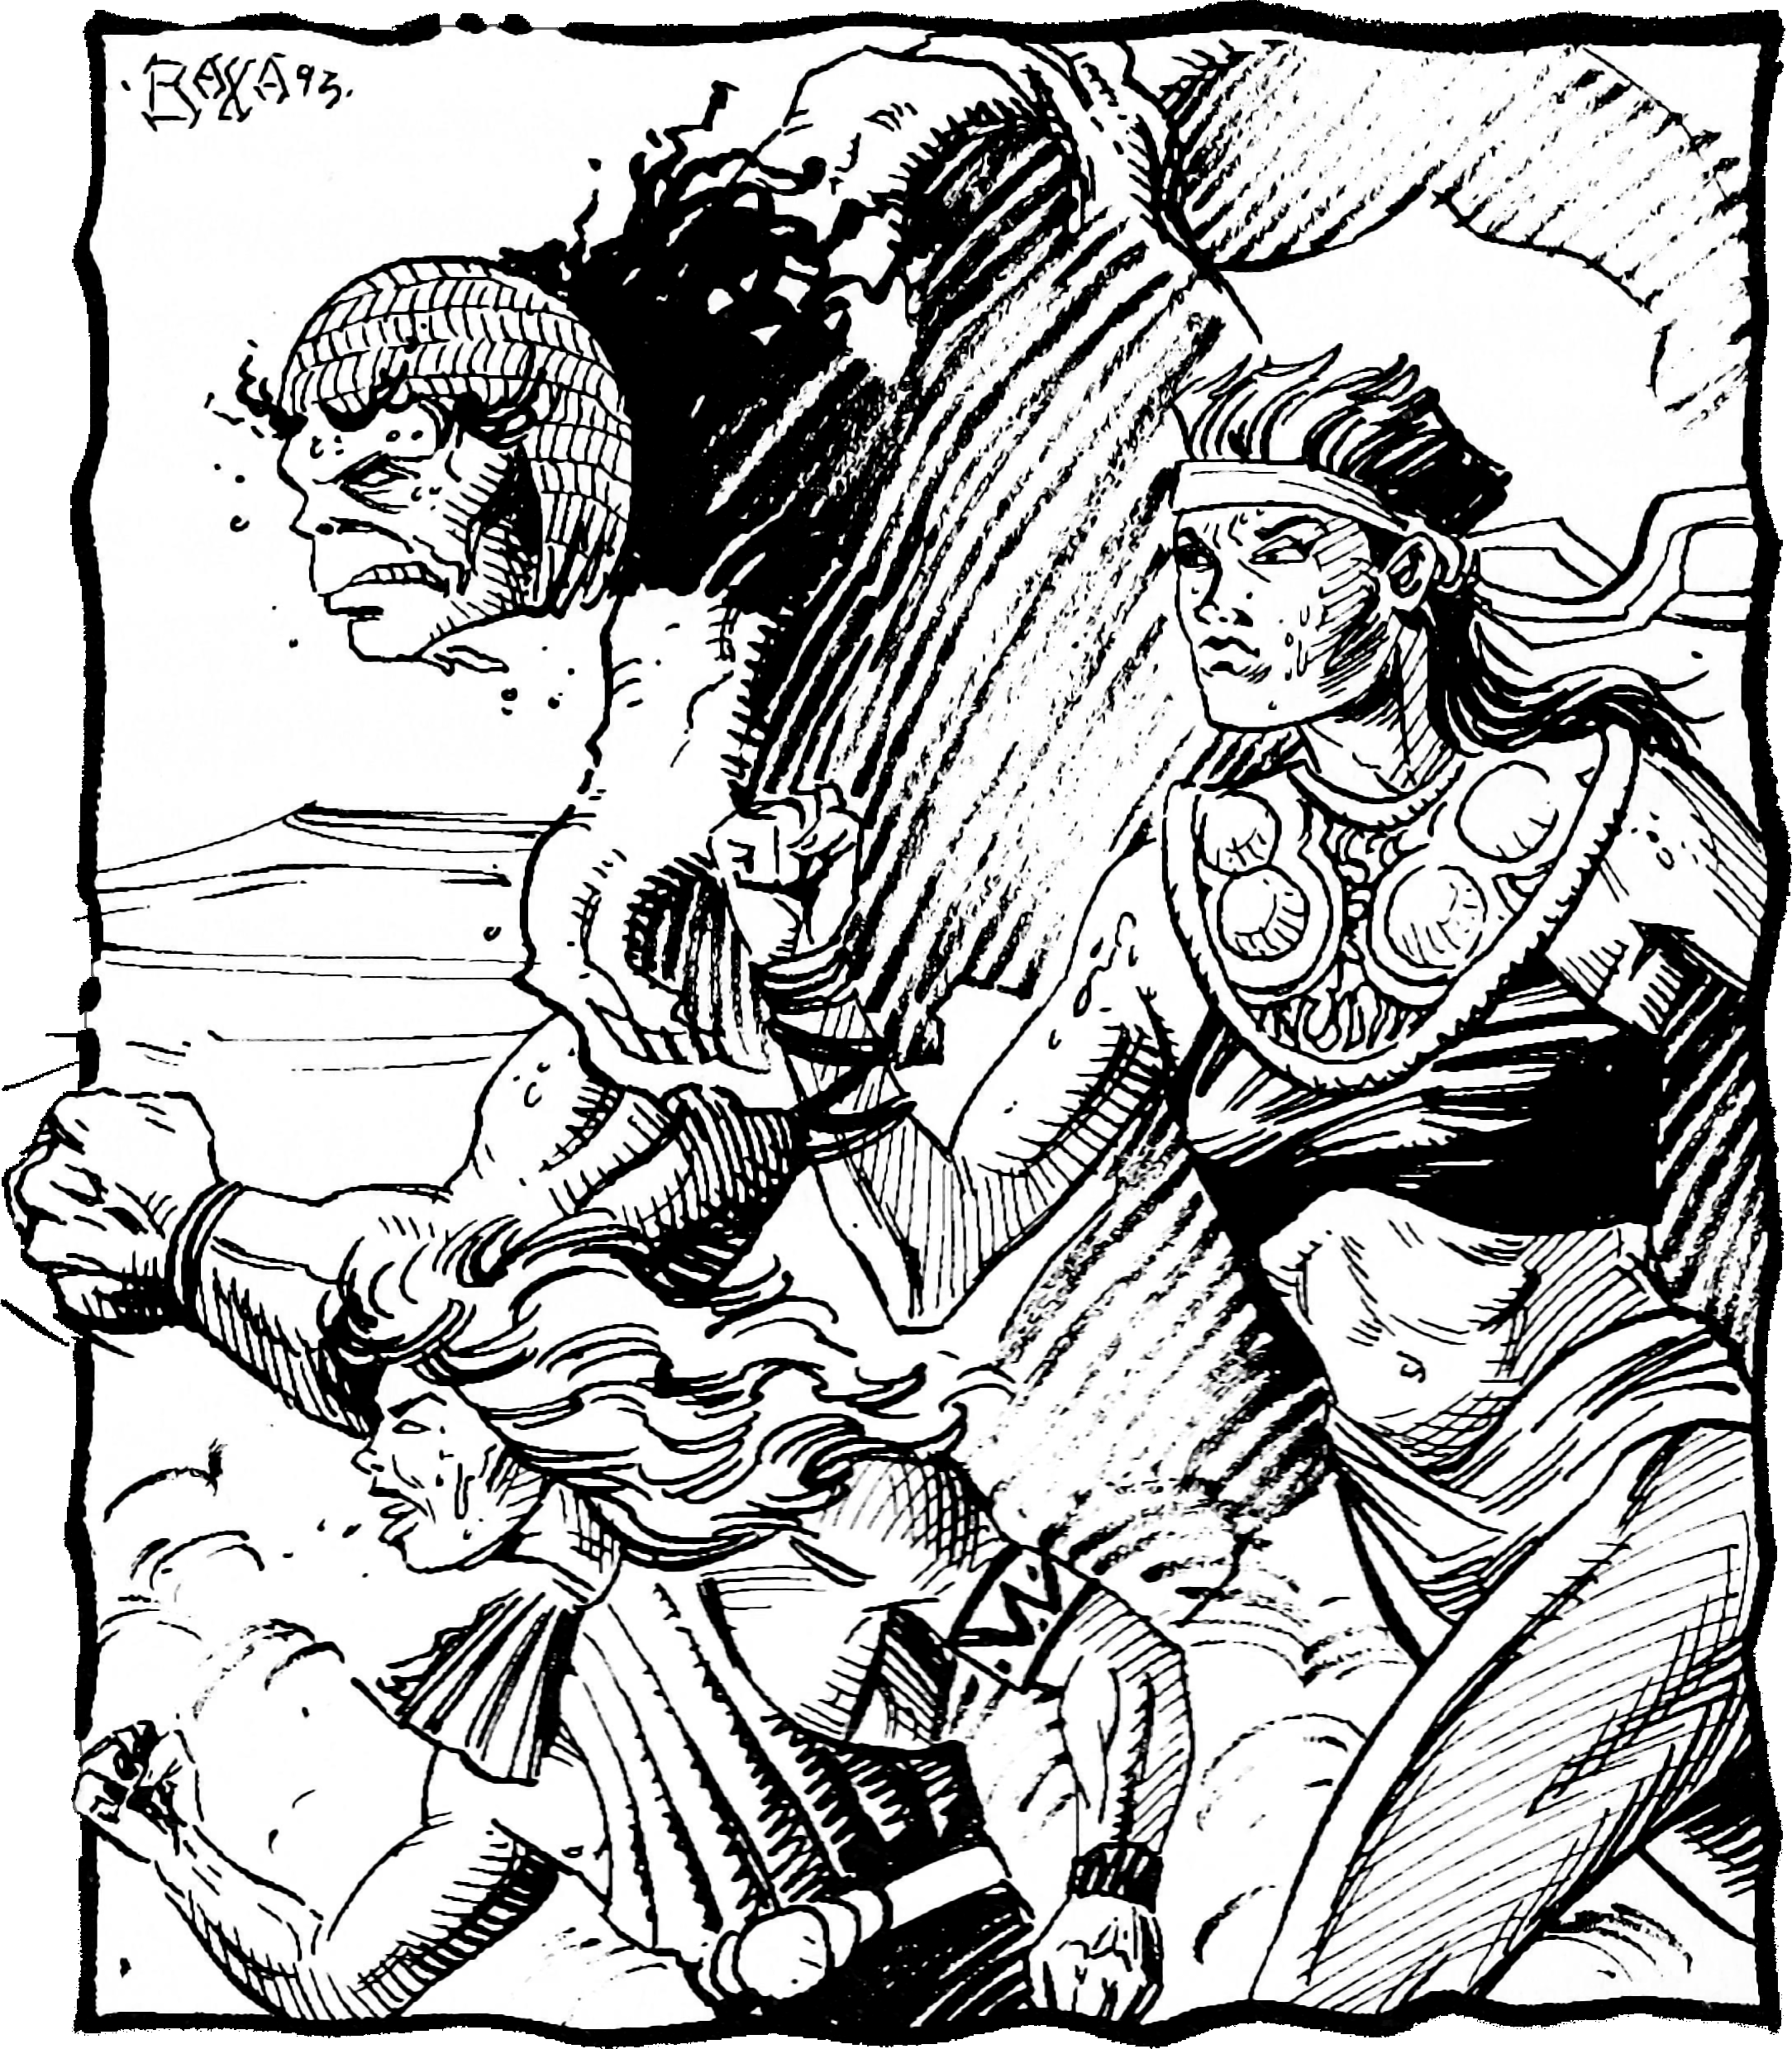
\includegraphics[width=\columnwidth]{images/running-1.png}
\WOTC
\end{figure}
\subsubsection{Run}
You can run as a full-round action. (If you do, you do not also get a 1.5-meter step.) When you run, you can move up to four times your speed in a straight line (or three times your speed if you're in heavy armor). You lose any Dexterity bonus to AC unless you have the \feat{Run} feat.

You can run for a number of rounds equal to your Constitution score, but after that you must make a DC 10 Constitution check to continue running. You must check again each round in which you continue to run, and the DC of this check increases by 1 for each check you have made. When you fail this check, you must stop running. A character who has run to his limit must rest for 1 minute (10 rounds) before running again. During a rest period, a character can move no faster than a normal move action.

You can't run across difficult terrain or if you can't see where you're going.

A run represents a speed of about 18 kilometers per hour for an unencumbered human.

\subsubsection{Move 1.5 meter through Difficult Terrain}
In some situations, your movement may be so hampered that you don't have sufficient speed even to move 1.5 meter (a single square). In such a case, you may spend a full-round action to move 1.5 meter (1 square) in any direction, even diagonally. Even though this looks like a 1.5-meter step, it's not, and thus it provokes attacks of opportunity normally.
\subsection{Free Actions}
\Table{Free Actions}{LZ{14mm}}{
\tableheader Action & \tableheader Attack of Opportunity\footnotemark[1] \\
Cease concentration on a spell & No \\
Drop an item & No \\
Drop to the floor & No \\
Prepare spell components to cast a spell\footnotemark[2] & No \\
Speak & No \\
\TableNote{2}{1 Regardless of the action, if you move out of a threatened square, you usually provoke an attack of opportunity. This column indicates whether the action itself, not moving, provokes an attack of opportunity.}\\
\TableNote{2}{2 Unless the component is an extremely large or awkward item.}\\
}

Free actions don't take any time at all, though there may be limits to the number of free actions you can perform in a turn. Free actions rarely incur attacks of opportunity. Some common free actions are described below.

\subsubsection{Drop an Item}
Dropping an item in your space or into an adjacent square is a free action.

\subsubsection{Drop Prone}
Dropping to a prone position in your space is a free action.

\subsubsection{Speak}
In general, speaking is a free action that you can perform even when it isn't your turn. Speaking more than few sentences is generally beyond the limit of a free action.

\subsubsection{Cease Concentration on Spell}
You can stop concentrating on an active spell as a free action.

\Table{Swift Actions}{LZ{14mm}}{
\tableheader Action & \tableheader Attack of Opportunity\footnotemark[1] \\
Assume stance & No \\
Cast quickened spell & No \\
Cast spell (1 swift action casting time) & No \\
Use gladiatorial performance & No \\
Use quickened spell-like ability & No \\
\TableNote{2}{1 Regardless of the action, if you move out of a threatened square, you usually provoke an attack of opportunity. This column indicates whether the action itself, not moving, provokes an attack of opportunity.}\\
}

\subsection{Swift Actions}
A swift action consumes a very small amount of time, but represents a larger expenditure of effort and energy than a free action. You can perform one swift action per turn without affecting your ability to perform other actions. In that regard, a swift action is like a free action. However, you can perform only a single swift action per turn, regardless of what other actions you take. You can take a swift action any time you would normally be allowed to take a free action. Swift actions usually involve spellcasting or the activation of magic items; many characters (especially those who don't cast spells) never have an opportunity to take a swift action.

Casting a quickened spell is a swift action. In addition, casting any spell with a casting time of 1 swift action is a swift action.

Casting a spell with a casting time of 1 swift action does not provoke attacks of opportunity.

\subsection{Immediate Actions}
\Table{Immediate Actions}{LZ{14mm}}{
  \tableheader Action
& \tableheader Attack of Opportunity\footnotemark[1] \\
Cast spell (1 immediate action casting time) & No \\
Use the \feat{Greater Counterspell} feat     & Yes \\
Use martial prowess                          & No \\
\TableNote{2}{1 Regardless of the action, if you move out of a threatened square, you usually provoke an attack of opportunity. This column indicates whether the action itself, not moving, provokes an attack of opportunity.}\\
}

Much like a swift action, an immediate action consumes a very small amount of time, but represents a larger expenditure of effort and energy than a free action. However, unlike a swift action, an immediate action can be performed at any time---even if it's not your turn. An immediate action is an instant response to a trigger of some kind. For example, an attack, a spell cast, a successful hit, or enemy reaching a specific spot.

Casting \spell{feather fall} is an immediate action, since the spell can be cast at any time.

Using an immediate action on your turn is the same as using a swift action, and counts as your swift action for that turn. You cannot use another immediate action or a swift action until after your next turn if you have used an immediate action when it is not currently your turn (effectively, using an immediate action before your turn is equivalent to using your swift action for the coming turn). You also cannot use an immediate action if you are flat-footed.

\subsection{Miscellaneous Actions}
\Table{Miscellaneous Actions}{LZ{14mm}}{
  \tableheader No Action
& \tableheader Attack of Opportunity\footnotemark[1] \\
1.5-meter step                                    & No \\
Delay                                             & No \\
Fight defensively                                 & No \\
Make \skill{Concentration} check                  & No \\
Make passive \skill{Listen} or \skill{Spot} check & No \\

% \cmidrule[0pt]{1-2}

  \tableheader Action Type Varies
& \tableheader Attack of Opportunity\footnotemark[1] \\
Disarm\footnotemark[2]           & Yes \\
Grapple\footnotemark[2]          & Yes \\
Trip an opponent\footnotemark[2] & Yes \\
Use feat\footnotemark[3]         & Varies \\

\TableNote{2}{1 Regardless of the action, if you move out of a threatened square, you usually provoke an attack of opportunity. This column indicates whether the action itself, not moving, provokes an attack of opportunity.}\\
\TableNote{2}{2 These attack forms substitute for a melee attack, not an action. As melee attacks, they can be used once in an attack or charge action, one or more times in a full attack action, or even as an attack of opportunity.}\\
\TableNote{2}{3 The description of a feat defines its effect.}\\
}

\subsubsection{Take 1.5-Meter Step}
You can move 1.5 meter in any round when you don't perform any other kind of movement. Taking this 1.5-meter step never provokes an attack of opportunity. You can't take more than one 1.5-meter step in a round, and you can't take a 1.5-meter step in the same round when you move any distance.

You can take a 1.5-meter step before, during, or after your other actions in the round.

You can only take a 1.5-meter step if your movement isn't hampered by difficult terrain or darkness. Any creature with a speed of 1.5 meter or less can't take a 1.5-meter step, since moving even 1.5 meter requires a move action for such a slow creature.

You may not take a 1.5-meter step using a form of movement for which you do not have a listed speed.

\subsubsection{Use Feat}
Certain feats let you take special actions in combat. Other feats do not require actions themselves, but they give you a bonus when attempting something you can already do. Some feats are not meant to be used within the framework of combat. The individual feat descriptions tell you what you need to know about them.

\subsubsection{Use Skill}
Most skill uses are standard actions, but some might be move actions, full-round actions, free actions, or something else entirely.

The individual skill descriptions tell you what sorts of actions are required to perform skills.


\begin{figure*}[b!]
\centering
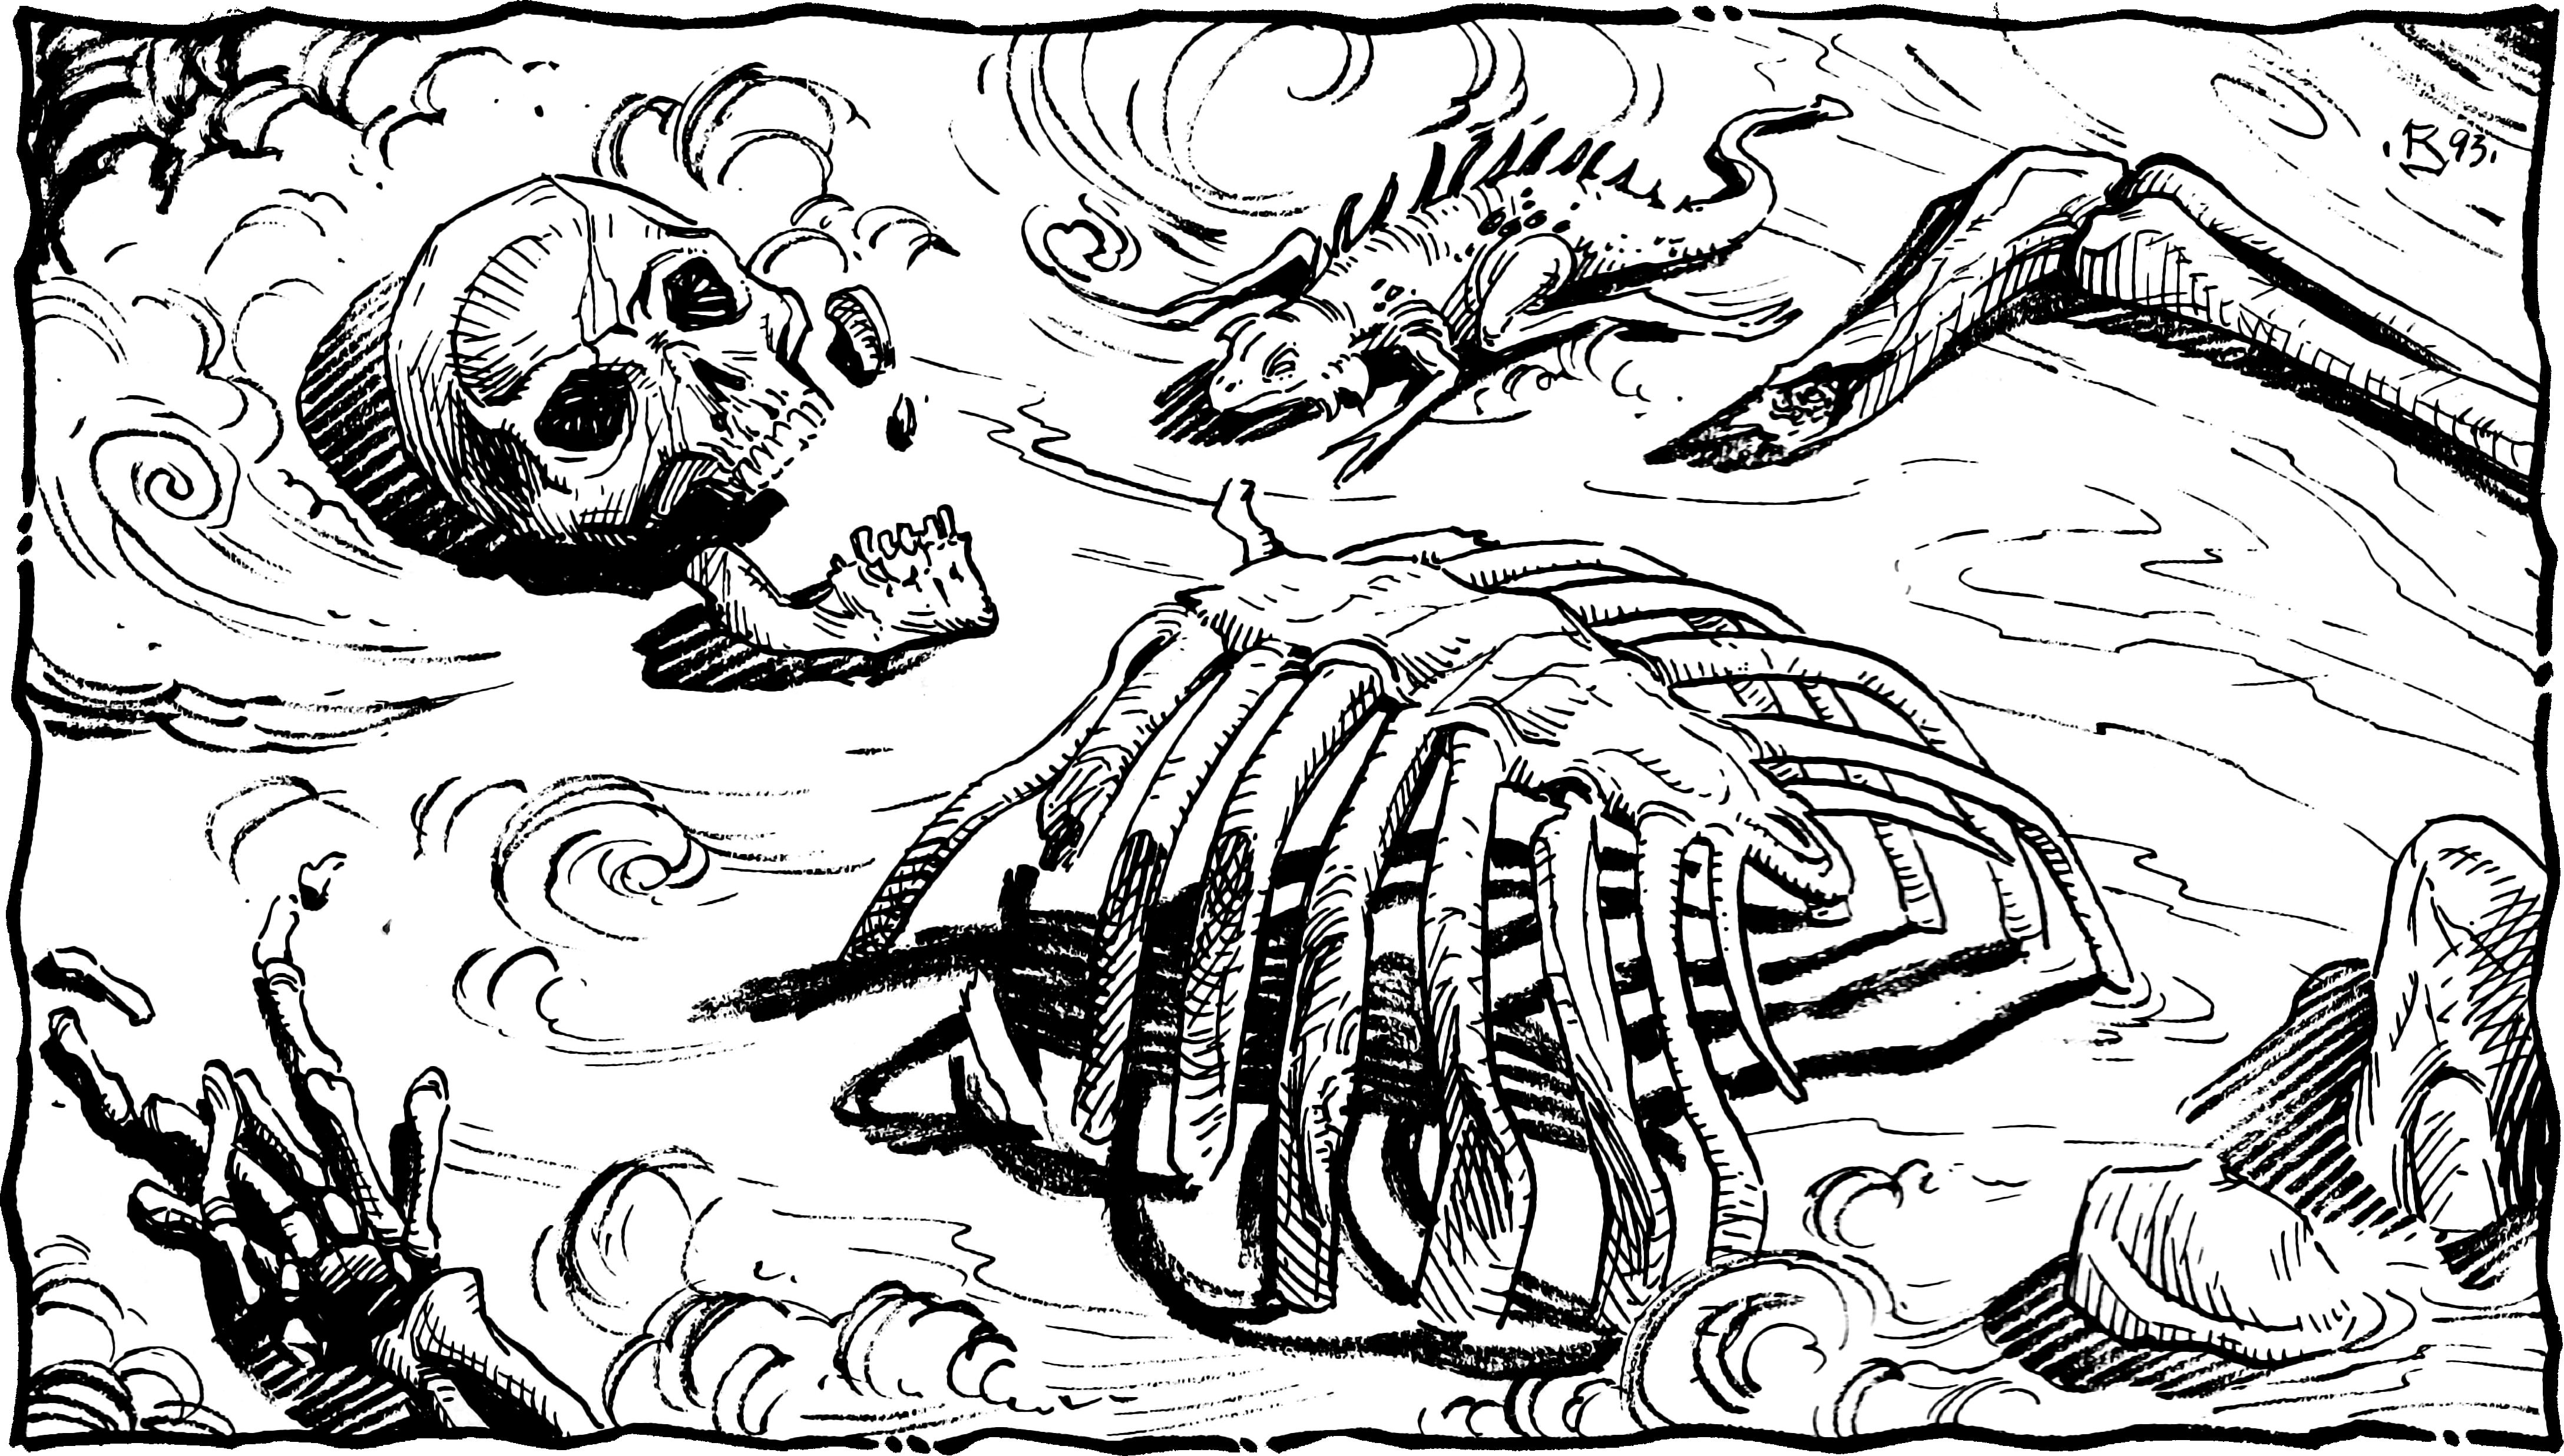
\includegraphics[width=\textwidth]{images/skeleton-1.png}
\WOTC
\end{figure*}
\section{Injury and Death}
Your hit points measure how hard you are to kill. No matter how many hit points you lose, your character isn't hindered in any way until your hit points drop to 0 or lower.

\subsection{Loss Of Hit Points}
The most common way that your character gets hurt is to take lethal damage and lose hit points.

\textbf{What Hit Points Represent:} Hit points mean two things in the game world: the ability to take physical punishment and keep going, and the ability to turn a serious blow into a less serious one.

\textbf{Effects of Hit Point Damage:} Damage doesn't slow you down until your current hit points reach 0 or lower. At 0 hit points, you're disabled.

At from $-1$ to $-9$ hit points, you're dying.

At $-10$ or lower, you're dead.

\textbf{Massive Damage:} If you ever sustain a single attack deals 50 points of damage or more and it doesn't kill you outright, you must make a DC 15 Fortitude save. If this saving throw fails, you die regardless of your current hit points. If you take 50 points of damage or more from multiple attacks, no one of which dealt 50 or more points of damage itself, the massive damage rule does not apply.

\subsection{Disabled (0 Hit Points)}
When your current hit points drop to exactly 0, you're disabled.

You can only take a single move or standard action each turn (but not both, nor can you take full$-round$ actions). You can take move actions without further injuring yourself, but if you perform any standard action (or any other strenuous action) you take 1 point of damage after the completing the act. Unless your activity increased your hit points, you are now at $-1$ hit points, and you're dying.

Healing that raises your hit points above 0 makes you fully functional again, just as if you'd never been reduced to 0 or fewer hit points.

You can also become disabled when recovering from dying. In this case, it's a step toward recovery, and you can have fewer than 0 hit points (see Stable Characters and Recovery, below).

\subsection{Dying ($-1$ to $-9$ Hit Points)}
When your character's current hit points drop to between $-1$ and $-9$ inclusive, he's dying.

A dying character immediately falls unconscious and can take no actions.

A dying character loses 1 hit point every round. This continues until the character dies or becomes stable (see below).

\subsection{Dead ($-10$ Hit Points or Lower)}
When your character's current hit points drop to $-10$ or lower, or if he takes massive damage (see above), he's dead. A character can also die from taking ability damage or suffering an ability drain that reduces his Constitution to 0.

\begin{figure*}[t!]
\centering
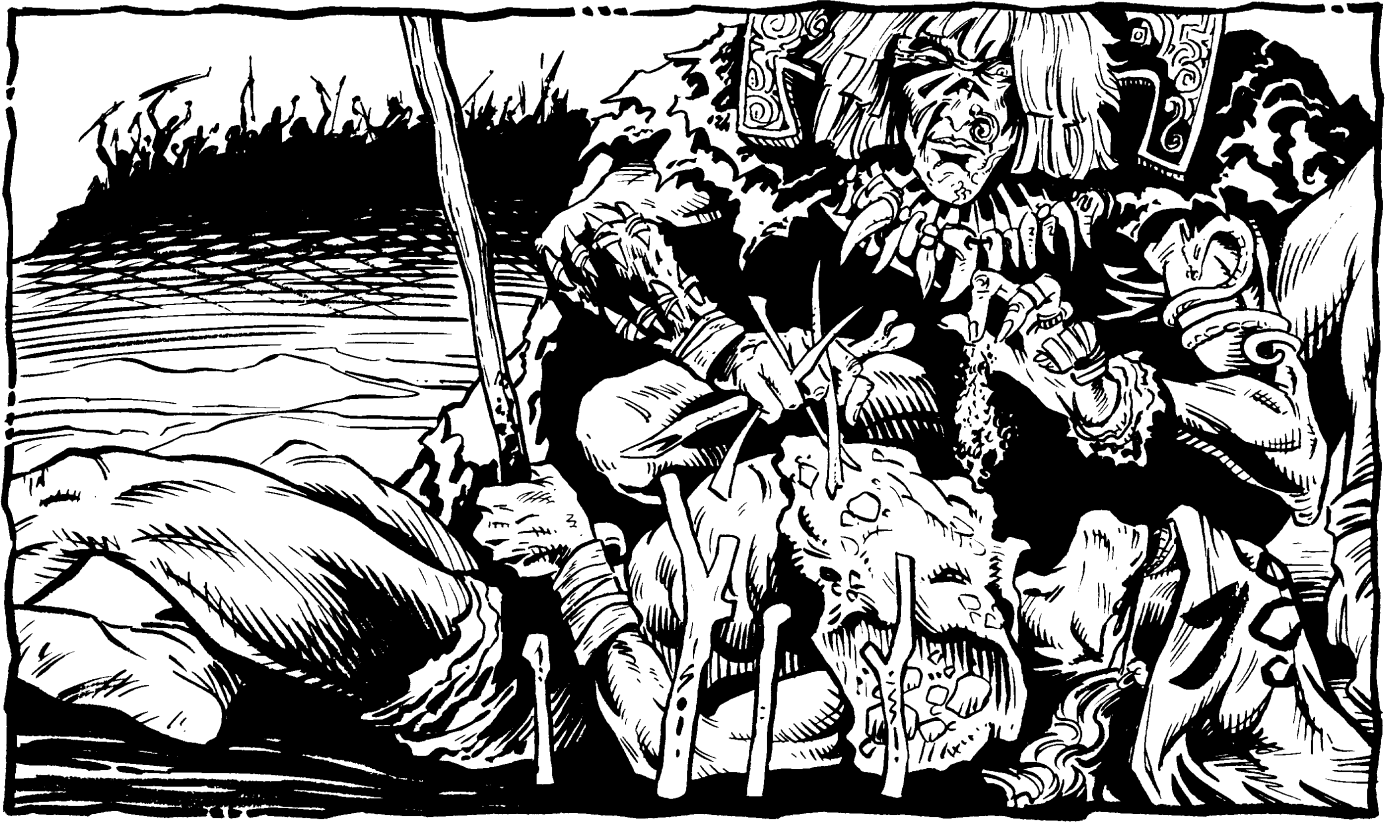
\includegraphics[width=\textwidth]{images/heal-1.png}
\WOTC
\end{figure*}
\subsection{Stable Characters and Recovery}
On the next turn after a character is reduced to between $-1$ and $-9$ hit points and on all subsequent turns, roll d\% to see whether the dying character becomes stable. He has a 10\% chance of becoming stable. If he doesn't, he loses 1 hit point. (A character who's unconscious or dying can't use any special action that changes the initiative count on which his action occurs.)

If the character's hit points drop to $-10$ or lower, he's dead.

You can keep a dying character from losing any more hit points and make him stable with a DC 15 \skill{Heal} check.

If any sort of healing cures the dying character of even 1 point of damage, he stops losing hit points and becomes stable.

Healing that raises the dying character's hit points to 0 makes him conscious and disabled. Healing that raises his hit points to 1 or more makes him fully functional again, just as if he'd never been reduced to 0 or lower. A spellcaster retains the spellcasting capability she had before dropping below 0 hit points.

A stable character who has been tended by a healer or who has been magically healed eventually regains consciousness and recovers hit points naturally. If the character has no one to tend him, however, his life is still in danger, and he may yet slip away.

\textbf{Recovering with Help:} One hour after a tended, dying character becomes stable, roll d\%. He has a 10\% chance of becoming conscious, at which point he is disabled (as if he had 0 hit points). If he remains unconscious, he has the same chance to revive and become disabled every hour. Even if unconscious, he recovers hit points naturally. He is back to normal when his hit points rise to 1 or higher.

\textbf{Recovering without Help:} A severely wounded character left alone usually dies. He has a small chance, however, of recovering on his own.

A character who becomes stable on his own (by making the 10\% roll while dying) and who has no one to tend to him still loses hit points, just at a slower rate. He has a 10\% chance each hour of becoming conscious. Each time he misses his hourly roll to become conscious, he loses 1 hit point. He also does not recover hit points through natural healing.

Even once he becomes conscious and is disabled, an unaided character still does not recover hit points naturally. Instead, each day he has a 10\% chance to start recovering hit points naturally (starting with that day); otherwise, he loses 1 hit point.

Once an unaided character starts recovering hit points naturally, he is no longer in danger of naturally losing hit points (even if his current hit point total is negative).

\subsection{Healing}
After taking damage, you can recover hit points through natural healing or through magical healing. In any case, you can't regain hit points past your full normal hit point total.

\textbf{Natural Healing:} With a full night's rest (8 hours of sleep or more), you recover 1 hit point per character level. Any significant interruption during your rest prevents you from healing that night.

If you undergo complete bed rest for an entire day and night, you recover twice your character level in hit points.

\textbf{Magical Healing:} Various abilities and spells can restore hit points.

\textbf{Healing Limits:} You can never recover more hit points than you lost. Magical healing won't raise your current hit points higher than your full normal hit point total.

\textbf{Healing Ability Damage:} Ability damage is temporary, just as hit point damage is. Ability damage returns at the rate of 1 point per night of rest (8 hours) for each affected ability score. Complete bed rest restores 2 points per day (24 hours) for each affected ability score.

\subsection{Temporary Hit Points}
Certain effects give a character temporary hit points. When a character gains temporary hit points, note his current hit point total. When the temporary hit points go away the character's hit points drop to his current hit point total. If the character's hit points are below his current hit point total at that time, all the temporary hit points have already been lost and the character's hit point total does not drop further.

When temporary hit points are lost, they cannot be restored as real hit points can be, even by magic.

\textbf{Increases in Constitution Score and Current Hit Points:} An increase in a character's Constitution score, even a temporary one, can give her more hit points (an effective hit point increase), but these are not temporary hit points. They can be restored and they are not lost first as temporary hit points are.

\subsection{Nonlethal Damage}
\textbf{Dealing Nonlethal Damage:} Certain attacks deal nonlethal damage. Other effects, such as heat or being exhausted, also deal nonlethal damage. When you take nonlethal damage, keep a running total of how much you've accumulated. Do not deduct the nonlethal damage number from your current hit points. It is not "real" damage. Instead, when your nonlethal damage equals your current hit points, you're staggered, and when it exceeds your current hit points, you fall unconscious. It doesn't matter whether the nonlethal damage equals or exceeds your current hit points because the nonlethal damage has gone up or because your current hit points have gone down.

\textit{Nonlethal Damage with a Weapon that Deals Lethal Damage:} You can use a melee weapon that deals lethal damage to deal nonlethal damage instead, but you take a $-4$ penalty on your attack roll.

\textit{Lethal Damage with a Weapon that Deals Nonlethal Damage:} You can use a weapon that deals nonlethal damage, including an unarmed strike, to deal lethal damage instead, but you take a $-4$ penalty on your attack roll.

\textbf{Staggered and Unconscious:} When your nonlethal damage equals your current hit points, you're staggered. You can only take a standard action or a move action in each round. You cease being staggered when your current hit points once again exceed your nonlethal damage.

When your nonlethal damage exceeds your current hit points, you fall unconscious. While unconscious, you are helpless.

Spellcasters who fall unconscious retain any spellcasting ability they had before going unconscious.

\textbf{Healing Nonlethal Damage:} You heal nonlethal damage at the rate of 1 hit point per hour per character level.

When a spell or a magical power cures hit point damage, it also removes an equal amount of nonlethal damage.


\section{Movement and Distance}
% \section{Movement, Position, and Distance}
Miniatures are on the 30mm scale---a miniature figure of a 1.8-meter-tall human is approximately 30mm tall. A square on the battle grid is 2.5 centimeters across, representing a 1.5-meter-by-1.5-meter area.

\subsection{Tactical Movement}
The characteristics of moving in a combat situation: distance to be covered, the possible impediments, and special rules are described below.


\Figure*{t}{images/kirre.png}

\subsubsection{How Far Can Your Character Move?}
Your speed is determined by your race and your armor (see \tabref{Tactical Speed}). Your speed while unarmored is your base land speed.

\textbf{Encumbrance:} A character encumbered by carrying a large amount of gear, treasure, or fallen comrades may move slower than normal.

\textbf{Hampered Movement:} Difficult terrain, obstacles, or poor visibility can hamper movement.

\textbf{Movement in Combat:} Generally, you can move your speed in a round and still do something (take a move action and a standard action).

If you do nothing but move (that is, if you use both of your actions in a round to move your speed), you can move double your speed.

If you spend the entire round running, you can move quadruple your speed. If you do something that requires a full round you can only take a 1.5-meter step.

\textbf{Bonuses to Speed:} A barbarian has a +3 meters bonus to his speed (unless he's wearing heavy armor). In addition, many spells and magic items can affect a character's speed. Always apply any modifiers to a character's speed before adjusting the character's speed based on armor or encumbrance, and remember that multiple bonuses of the same type to a character's speed don't stack.

\Table{Tactical Speed}{y{33mm}CC}{
  \tableheader Race
& \tableheader No Armor or Light Armor
& \tableheader Medium or Heavy Armor \\
Half-giant, thri-kreen    & 12m(8 squares) & 9m(6 squares) \\
Elf, Human, half-elf, mul & 9m(6 squares)  & 6m(4 squares) \\
Dwarf                     & 6m(4 squares)  & 6m(4 squares) \\
Halfling                  & 6m(4 squares)  & 4.5m(3 squares) \\
}

\subsubsection{Measuring Distance}
\textbf{Diagonals:} When measuring distance, the first diagonal counts as 1 square, the second counts as 2 squares, the third counts as 1, the fourth as 2, and so on.

You can't move diagonally past a corner (even by taking a 1.5-meter step). You can move diagonally past a creature, even an opponent.

You can also move diagonally past other impassable obstacles, such as pits.

\textbf{Closest Creature:} When it's important to determine the closest square or creature to a location, if two squares or creatures are equally close, randomly determine which one counts as closest by rolling a die.

\subsubsection{Moving through a Square}
\textbf{Friend:} You can move through a square occupied by a friendly character, unless you are charging. When you move through a square occupied by a friendly character, that character doesn't provide you with cover.

\textbf{Opponent:} You can't move through a square occupied by an opponent, unless the opponent is helpless. You can move through a square occupied by a helpless opponent without penalty. (Some creatures, particularly very large ones, may present an obstacle even when helpless. In such cases, each square you move through counts as 2 squares.)

\textbf{Ending Your Movement:} You can't end your movement in the same square as another creature unless it is helpless.

\textbf{Overrun:} During your movement you can attempt to move through a square occupied by an opponent.

\textbf{Tumbling:} A trained character can attempt to tumble through a square occupied by an opponent (see the Tumble skill).

\textbf{Very Small Creature:} A Fine, Diminutive, or Tiny creature can move into or through an occupied square. The creature provokes attacks of opportunity when doing so.

\textbf{Square Occupied by Creature Three Sizes Larger or Smaller:} Any creature can move through a square occupied by a creature three size categories larger than it is.

A big creature can move through a square occupied by a creature three size categories smaller than it is.

\textbf{Designated Exceptions:} Some creatures break the above rules. A creature that completely fills the squares it occupies cannot be moved past, even with the Tumble skill or similar special abilities.
\subsubsection{Terrain and Obstacles}
\textbf{Difficult Terrain:} Difficult terrain hampers movement. Each square of difficult terrain counts as 2 squares of movement. (Each diagonal move into a difficult terrain square counts as 3 squares.) You can't run or charge across difficult terrain.

If you occupy squares with different kinds of terrain, you can move only as fast as the most difficult terrain you occupy will allow.

Flying and incorporeal creatures are not hampered by difficult terrain.

\textbf{Obstacles:} Like difficult terrain, obstacles can hamper movement. If an obstacle hampers movement but doesn't completely block it each obstructed square or obstacle between squares counts as 2 squares of movement. You must pay this cost to cross the barrier, in addition to the cost to move into the square on the other side. If you don't have sufficient movement to cross the barrier and move into the square on the other side, you can't cross the barrier. Some obstacles may also require a skill check to cross.

On the other hand, some obstacles block movement entirely. A character can't move through a blocking obstacle.

Flying and incorporeal creatures can avoid most obstacles.

\textbf{Squeezing:} In some cases, you may have to squeeze into or through an area that isn't as wide as the space you take up. You can squeeze through or into a space that is at least half as wide as your normal space. Each move into or through a narrow space counts as if it were 2 squares, and while squeezed in a narrow space you take a $-4$ penalty on attack rolls and a $-4$ penalty to AC.

When a Large creature (which normally takes up four squares) squeezes into a space that's one square wide, the creature's miniature figure occupies two squares, centered on the line between the two squares. For a bigger creature, center the creature likewise in the area it squeezes into.

A creature can squeeze past an opponent while moving but it can't end its movement in an occupied square.

To squeeze through or into a space less than half your space's width, you must use the \skill{Escape Artist} skill. You can't attack while using \skill{Escape Artist} to squeeze through or into a narrow space, you take a $-4$ penalty to AC, and you lose any Dexterity bonus to AC.


\BigTableBottom{Creature Size and Scale}{l*{3}{Z{12mm}}XX*{3}{Z{14mm}}}{
\tableheader Size Category &
\tableheader Size\footnotemark[1] Modifier &
\tableheader Grapple\footnotemark[2] Modifier &
\tableheader Hide\footnotemark[3] Modifier &
\tableheader Height or Length\footnotemark[4] &
\tableheader Weight\footnotemark[5] &
\tableheader Space\footnotemark[6] &
\tableheader Natural Reach\footnotemark[6] (Tall) &
\tableheader Natural Reach\footnotemark[6] (Long)\\

Fine       & +8   & $-16$ & +16   & 15 cm or less  & 60 g or less        & 15 cm & 0 m   & 0 m   \\
Diminutive & +4   & $-12$ & +12   & 15 cm--30 cm   & 60 g--0.5 kg        & 30 cm & 0 m   & 0 m   \\
Tiny       & +2   & $-8$  & +8    & 30 cm--60 cm   & 0.5 kg--4 kg        & 75 cm & 0 m   & 0 m   \\
Small      & +1   & $-4$  & +4    & 60 cm--1.2 m   & 4 kg--30 kg         & 1.5 m & 1.5 m & 1.5 m \\
Medium     & +0   & +0    & +0    & 1.2 m--2.5 m   & 30 kg--250 kg       & 1.5 m & 1.5 m & 1.5 m \\
Large      & $-1$ & +4    & $-4$  & 2.5 m--5 m   & 250 kg--1 tonne     & 3 m   & 3 m   & 1.5 m \\
Huge       & $-2$ & +8    & $-8$  & 5 m--10 m   & 1 tonne--8 tonnes   & 4.5 m & 4.5 m & 3 m   \\
Gargantuan & $-4$ & +12   & $-12$ & 10 m--20 m  & 8 tonnes--60 tonnes & 6 m   & 6 m   & 4.5 m \\
Colossal   & $-8$ & +16   & $-16$ & 20 m or more & 60 tonnes or more   & 9 m   & 9 m   & 6 m   \\

\BigTableNote{9}{1 A creature's size modifier is applied to it's attack bonus and Armor Class.}\\
\BigTableNote{9}{2 See the Grapple special attack.}\\
\BigTableNote{9}{3 See the \skill{Hide} skill.}\\
\BigTableNote{9}{4 Biped's height, quadruped's body length (nose to base of tail)}\\
\BigTableNote{9}{5 Assumes that the creature is roughly as dense as a regular animal. A creature made of stone will weigh considerably more. A gaseous creature will weigh much less.}\\
\BigTableNote{9}{6 These values are typical for creatures of the indicated size. Some exceptions exist.}\\
}
\subsubsection{Special Movement Rules}
These rules cover special movement situations.

\textbf{Accidentally Ending Movement in an Illegal Space:} Sometimes a character ends its movement while moving through a space where it's not allowed to stop. When that happens, put your miniature in the last legal position you occupied, or the closest legal position, if there's a legal position that's closer.

\textbf{Double Movement Cost:} When your movement is hampered in some way, your movement usually costs double. For example, each square of movement through difficult terrain counts as 2 squares, and each diagonal move through such terrain counts as 3 squares (just as two diagonal moves normally do).

If movement cost is doubled twice, then each square counts as 4 squares (or as 6 squares if moving diagonally). If movement cost is doubled three times, then each square counts as 8 squares (12 if diagonal) and so on. This is an exception to the general rule that two doublings are equivalent to a tripling.

\textbf{Minimum Movement:} Despite penalties to movement, you can take a full-round action to move 1.5 meter (1 square) in any direction, even diagonally. (This rule doesn't allow you to move through impassable terrain or to move when all movement is prohibited.) Such movement provokes attacks of opportunity as normal (despite the distance covered, this move isn't a 1.5-meter step).

% \Figure*[\textwidth-22mm]{t}{images/sizes-1.png}

\subsection{Big and Little Creatures}
% \subsection{Big and Little Creatures In Combat}
Creatures smaller than Small or larger than Medium have special rules relating to position, reach, and weapon size.

\textbf{Tiny, Diminutive, and Fine Creatures:} Very small creatures take up less than 1 square of space. This means that more than one such creature can fit into a single square. A Tiny creature typically occupies a space only 75 centimeters across, so four can fit into a single square. Twenty-five Diminutive creatures or 100 Fine creatures can fit into a single square.

Creatures that take up less than 1 square of space typically have a natural reach of 0 meters, meaning they can't reach into adjacent squares. They must enter an opponent's square to attack in melee. This provokes an attack of opportunity from the opponent. You can attack into your own square if you need to, so you can attack such creatures normally.

Since they have no natural reach, they do not threaten the squares around them. You can move past them without provoking attacks of opportunity. They also can't flank an enemy.

\Figure{b}{images/sizes-1.png}
\textbf{Large, Huge, Gargantuan, and Colossal Creatures:} Very large creatures take up more than 1 square. For instance, a half-giant takes up a space 3 meters on a side (2 squares wide).

Creatures that take up more than 1 square typically have a natural reach of 3 meters or more, meaning that they can reach targets even if they aren't in adjacent squares.

Unlike when someone uses a reach weapon, a creature with greater than normal natural reach (more than 1.5 meter) still threatens squares adjacent to it. A creature with greater than normal natural reach usually gets an attack of opportunity against you if you approach it, because you must enter and move within the range of its reach before you can attack it. (This attack of opportunity is not provoked if you take a 1.5-meter step.)

Large or larger creatures using reach weapons can strike up to double their natural reach but can't strike at their natural reach or less.

\section{Combat Modifiers}
Sometimes you just have to go toe-to-toe in a fight, but you can usually gain some advantage by seeking a better position, either offensively or defensively. This section covers the rules for when you can line up a particularly good attack or are forced to make a disadvantageous one.

\subsection{(Un)Favorable Conditions}
% \subsection{Favorable and Unfavorable Conditions}
Depending on the condition of attackers or defenders, they may gain bonuses or penalties as stated in \tabref{Attack Roll Modifiers} and \tabref{Armor Class Modifiers}.

\Table{Attack Roll Modifiers}{Xcc}{
\tableheader Attacker is... & \tableheader Melee & \tableheader Ranged\\
Dazzled                   & $-1$                 & $-1$ \\
Entangled                 & $-2$\footnotemark[1] & $-2$\footnotemark[1] \\
Flanking defender         & Advantage            & --- \\
Invisible                 & +2\footnotemark[2]   & +2\footnotemark[2] \\
On higher ground          & +1                   & +0 \\
Prone                     & Disadvantage         & ---\footnotemark[3] \\
Shaken or frightened      & $-2$                 & $-2$ \\
Squeezing through a space & Disadvantage         & Disadvantage \\

\TableNote{3}{1 An entangled character also takes a $-4$ penalty to Dexterity, which may affect his attack roll.}\\
\TableNote{3}{2 The defender loses any Dexterity bonus to AC. This bonus doesn't apply if the target is blinded.}\\
\TableNote{3}{3 Most ranged weapons can't be used while the attacker is prone, but you can use a crossbow or shuriken while prone at no penalty.}\\
}

\Table{Armor Class Modifiers}{L*{2}{Z{12mm}}}{
\tableheader Defender is... & \tableheader Melee & \tableheader Ranged\\
Behind cover & +4 & +4 \\
Blinded & $-2$\footnotemark[1] & $-2$\footnotemark[1] \\
Concealed or invisible & \multicolumn{2}{c}{See Concealment} \\
Cowering & $-2$\footnotemark[1] & $-2$\footnotemark[1] \\
Entangled & +0\footnotemark[2] & +0\footnotemark[2] \\
Flat-footed (such as surprised, balancing, climbing) & +0\footnotemark[1] & +0\footnotemark[1] \\
Grappling (but attacker is not) & +0\footnotemark[1] & +0\footnotemark[1]\footnotemark[3] \\
Helpless (such as paralyzed, sleeping, or bound) & $-4$\footnotemark[4] & +0\footnotemark[4] \\
Kneeling or sitting & $-2$ & +2 \\
Pinned & $-4$\footnotemark[4] & +0\footnotemark[4] \\
Prone & $-4$ & +4 \\
Squeezing through a space & $-4$ & $-4$ \\
Stunned & -2\footnotemark[1] & -2\footnotemark[1] \\

\TableNote{3}{1 The defender loses any Dexterity bonus to AC.}\\
\TableNote{3}{2 An entangled character takes a $-4$ penalty to Dexterity.}\\
\TableNote{3}{3 Roll randomly to see which grappling combatant you strike. That defender loses any Dexterity bonus to AC.}\\
\TableNote{3}{4 Treat the defender's Dexterity as 0 ($-5$ modifier). Rogues can sneak attack helpless or pinned defenders.}\\
}

\begin{figure*}[t!]
\centering
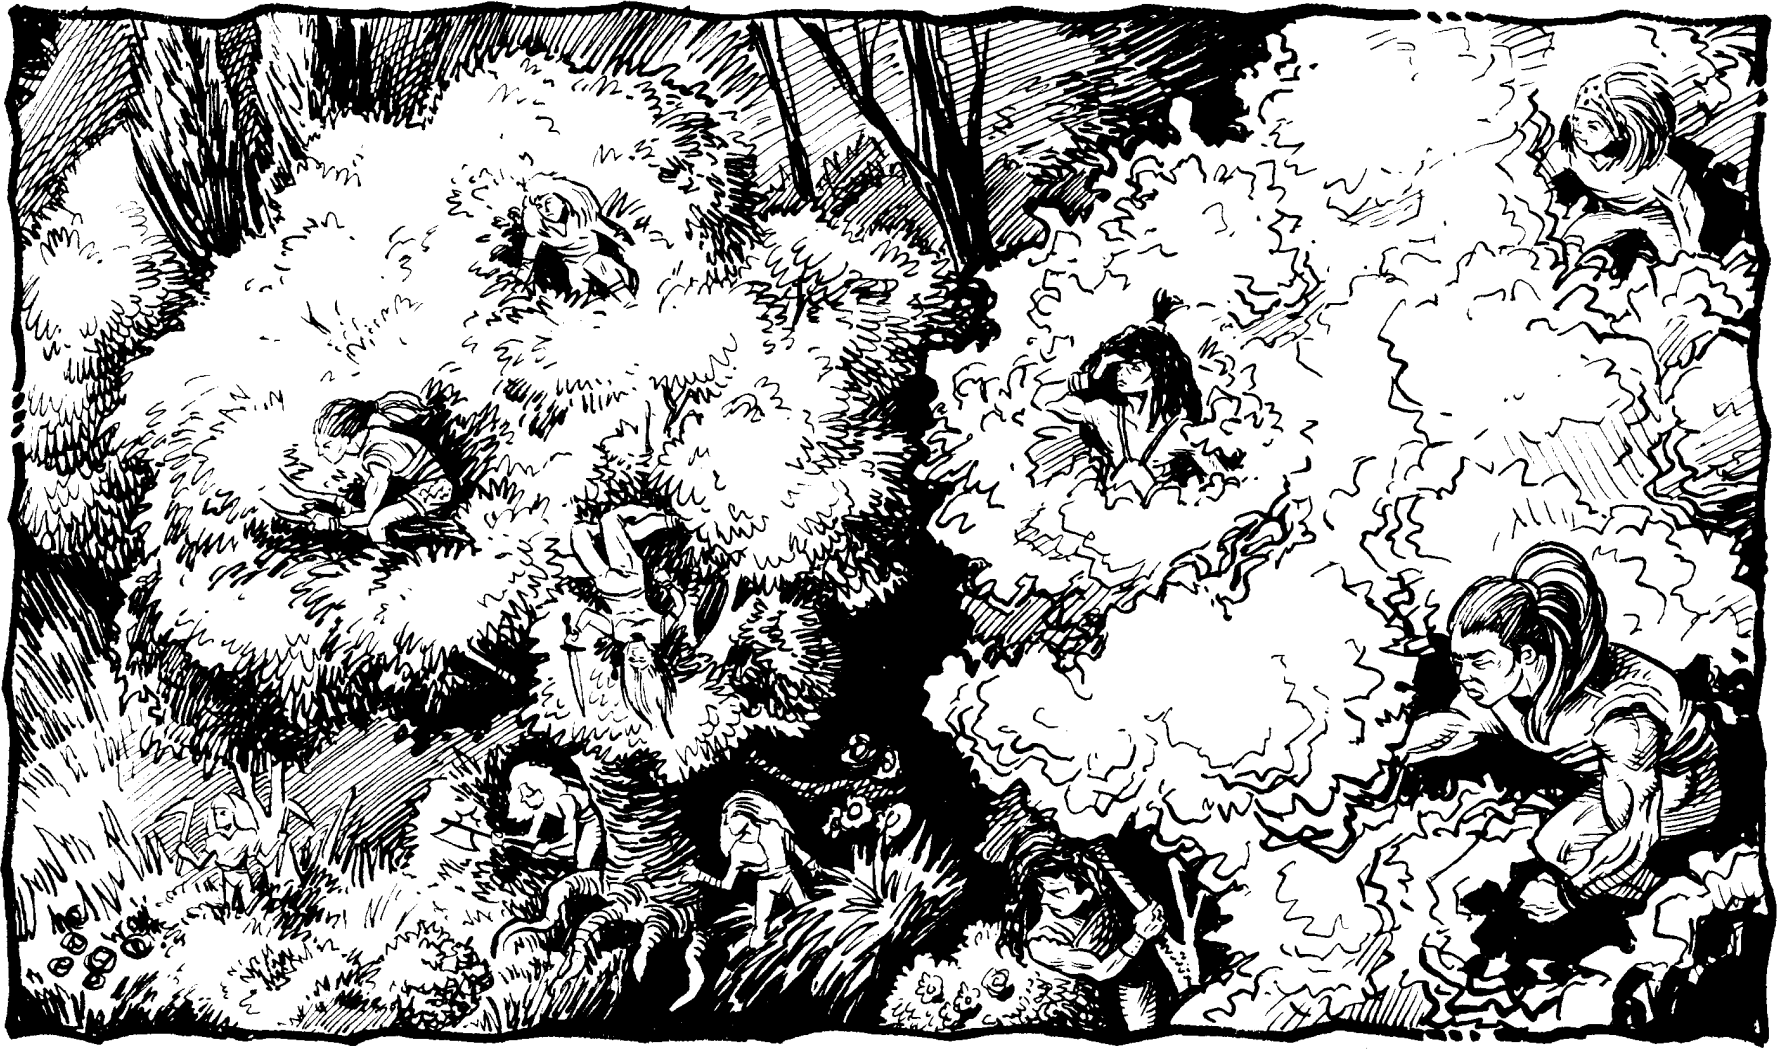
\includegraphics[width=\textwidth]{images/cover-1.png}
\WOTC
\end{figure*}
\subsection{Cover}
To determine whether your target has cover from your ranged attack, choose a corner of your square. If any line from this corner to any corner of the target's square passes through a square or border that blocks line of effect or provides cover, or through a square occupied by a creature, the target has cover (+4 to AC).

When making a melee attack against an adjacent target, your target has cover if any line from your square to the target's square goes through a wall (including a low wall). When making a melee attack against a target that isn't adjacent to you (such as with a reach weapon), use the rules for determining cover from ranged attacks.

\textbf{Low Obstacles and Cover:} A low obstacle (such as a wall no higher than half your height) provides cover, but only to creatures within 9 meters (6 squares) of it. The attacker can ignore the cover if he's closer to the obstacle than his target.

\textbf{Cover and Attacks of Opportunity:} You can't execute an attack of opportunity against an opponent with cover relative to you.

\textbf{Cover and Reflex Saves:} Cover grants you a +2 bonus on Reflex saves against attacks that originate or burst out from a point on the other side of the cover from you. Note that spread effects can extend around corners and thus negate this cover bonus.

\textbf{Cover and Hide Checks:} You can use cover to make a \skill{Hide} check. Without cover, you usually need concealment to make a \skill{Hide} check.

\textbf{Soft Cover:} Creatures, even your enemies, can provide you with cover against ranged attacks, giving you a +4 bonus to AC. However, such soft cover provides no bonus on Reflex saves, nor does soft cover allow you to make a \skill{Hide} check.

\textbf{Big Creatures and Cover:} Any creature with a space larger than 1.5 meter (1 square) determines cover against melee attacks slightly differently than smaller creatures do. Such a creature can choose any square that it occupies to determine if an opponent has cover against its melee attacks. Similarly, when making a melee attack against such a creature, you can pick any of the squares it occupies to determine if it has cover against you.

\textbf{Total Cover:} If you don't have line of effect to your target he is considered to have total cover from you. You can't make an attack against a target that has total cover.

\textbf{Varying Degrees of Cover:} In some cases, cover may provide a greater bonus to AC and Reflex saves. In such situations the normal cover bonuses to AC and Reflex saves can be doubled (to +8 and +4, respectively). A creature with this improved cover effectively gains improved evasion against any attack to which the Reflex save bonus applies. Furthermore, improved cover provides a +10 bonus on \skill{Hide} checks.
\subsection{Concealment}
To determine whether your target has concealment from your ranged attack, choose a corner of your square. If any line from this corner to any corner of the target's square passes through a square or border that provides concealment, the target has concealment.

When making a melee attack against an adjacent target, your target has concealment if his space is entirely within an effect that grants concealment. When making a melee attack against a target that isn't adjacent to you use the rules for determining concealment from ranged attacks.

In addition, some magical effects provide concealment against all attacks, regardless of whether any intervening concealment exists.

\textbf{Concealment Miss Chance:} Concealment gives the subject of a successful attack a 20\% chance that the attacker missed because of the concealment. If the attacker hits, the defender must make a miss chance percentile roll to avoid being struck. Multiple concealment conditions do not stack.

\textbf{Concealment and Hide Checks:} You can use concealment to make a Hide check. Without concealment, you usually need cover to make a Hide check.

\textbf{Total Concealment:} If you have line of effect to a target but not line of sight he is considered to have total concealment from you. You can't attack an opponent that has total concealment, though you can attack into a square that you think he occupies. A successful attack into a square occupied by an enemy with total concealment has a 50\% miss chance (instead of the normal 20\% miss chance for an opponent with concealment).

You can't execute an attack of opportunity against an opponent with total concealment, even if you know what square or squares the opponent occupies.

\textbf{Ignoring Concealment:} Concealment isn't always effective. A shadowy area or darkness doesn't provide any concealment against an opponent with darkvision. Characters with low-light vision can see clearly for a greater distance with the same light source than other characters. Although invisibility provides total concealment, sighted opponents may still make Spot checks to notice the location of an invisible character. An invisible character gains a +20 bonus on Hide checks if moving, or a +40 bonus on Hide checks when not moving (even though opponents can't see you, they might be able to figure out where you are from other visual clues).

\textbf{Varying Degrees of Concealment:} Certain situations may provide more or less than typical concealment, and modify the miss chance accordingly.
\subsection{Flanking}
When making a melee attack, you get a +2 flanking bonus if your opponent is threatened by a character or creature friendly to you on the opponent's opposite border or opposite corner.

When in doubt about whether two friendly characters flank an opponent in the middle, trace an imaginary line between the two friendly characters' centers. If the line passes through opposite borders of the opponent's space (including corners of those borders), then the opponent is flanked.

\textit{Exception:} If a flanker takes up more than 1 square, it gets the flanking bonus if any square it occupies counts for flanking.

Only a creature or character that threatens the defender can help an attacker get a flanking bonus.

Creatures with a reach of 0 feet can't flank an opponent.
\subsection{Helpless Defenders}
A helpless opponent is someone who is bound, sleeping, paralyzed, unconscious, or otherwise at your mercy.

\textbf{Regular Attack:} A helpless character takes a $-4$ penalty to AC against melee attacks, but no penalty to AC against ranged attacks.

A helpless defender can't use any Dexterity bonus to AC. In fact, his Dexterity score is treated as if it were 0 and his Dexterity modifier to AC as if it were $-5$ (and a rogue can sneak attack him).

\textbf{Coup de Grace:} As a full-round action, you can use a melee weapon to deliver a coup de grace to a helpless opponent. You can also use a bow or crossbow, provided you are adjacent to the target.

You automatically hit and score a critical hit. If the defender survives the damage, he must make a Fortitude save (DC 10 + damage dealt) or die. A rogue also gets her extra sneak attack damage against a helpless opponent when delivering a coup de grace.

Delivering a coup de grace provokes attacks of opportunity from threatening opponents.

You can't deliver a coup de grace against a creature that is immune to critical hits. You can deliver a coup de grace against a creature with total concealment, but doing this requires two consecutive full-round actions (one to ``find'' the creature once you've determined what square it's in, and one to deliver the coup de grace).

\subsection{Proficiencies}
A character who uses a weapon with which they are not proficient gets disadvantage on attack rolls.

A character who wears armor and/or uses a shield with which they are not proficient takes the armor's (and/or shield's) armor check penalty on attack rolls and on all Strength-based and Dexterity-based ability and skill checks. The penalty for nonproficiency with armor stacks with the penalty for nonproficiency with shields

Weapon, armor, or shield proficiency may be granted by the character's race, class or by the following feats:

\begin{itemize*}
\item \feat{Armor Proficiency (Light)}
\item \feat{Armor Proficiency (Medium)}
\item \feat{Armor Proficiency (Heavy)}
\item \feat{Exotic Weapon Proficiency}
\item \feat{Martial Weapon Proficiency}
\item \feat{Shield Proficiency}
\item \feat{Simple Weapon Proficiency}
\item \feat{Tower Shield Proficiency}
\end{itemize*}

\section{Special Attacks}
This section covers grappling, feinting, mounted combats, and all other forms of special attacks.

\Table{Special Attacks}{lX}{
\tableheader Special Attack & \tableheader Brief Description\\
Aid another         & Grant an ally advantage on attacks or give disadvantage on an enemy's\\
Bull rush           & Push an opponent back 1.5 meter or more\\
Charge              & Move up to twice your speed and attack with a +2 bonus\\
Disarm              & Knock a weapon from your opponent's hands, or grab a worn item\\
Feint               & Negate your opponent's Dex bonus to AC\\
Grapple             & Wrestle with an opponent\\
Mounted Combat      & Fight while riding your steed\\
Overrun             & Plow past or over an opponent as you move\\
Sunder              & Strike an opponent's weapon or shield\\
Throw splash weapon & Throw container of dangerous liquid at target\\
Trip                & Trip an opponent\\
Turn/rebuke undead  & Channel positive (or negative) energy to turn away (or awe) undead\\
Two-weapon fighting & Fight with a weapon in each hand\\
}
\subsection{Aid Another}
In melee combat, you can help a friend attack or defend by distracting or interfering with an opponent. If you're in position to make a melee attack on an opponent that is engaging a friend in melee combat, you can attempt to aid your friend as a standard action. You make an attack roll against AC 10. If you succeed, your friend gains either gains advantage on his next attack roll against that opponent or that opponent has disadvantage on their next attack against your friend (your choice), as long as that attack comes before the beginning of your next turn. Multiple characters can aid the same friend, and similar bonuses stack.

You can also use this standard action to help a friend in other ways, such as when he is affected by a spell, or to assist another character's skill check.
\subsection{Bull Rush}
You can make a bull rush as a standard action (an attack) or as part of a charge. When you make a bull rush, you attempt to push an opponent straight back instead of damaging him. You can only bull rush an opponent who is one size category larger than you, the same size, or smaller.

\textbf{Initiating a Bull Rush:} First, you move into the defender's space. Doing this provokes an attack of opportunity from each opponent that threatens you, including the defender. (If you have the \feat{Improved Bull Rush} feat, you don't provoke an attack of opportunity from the defender.) Any attack of opportunity made by anyone other than the defender against you during a bull rush has a 25\% chance of accidentally targeting the defender instead, and any attack of opportunity by anyone other than you against the defender likewise has a 25\% chance of accidentally targeting you. (When someone makes an attack of opportunity, make the attack roll and then roll to see whether the attack went astray.)

Second, you and the defender make opposed Strength checks. You each add a +4 bonus for each size category you are larger than Medium or a $-4$ penalty for each size category you are smaller than Medium. You get advantage on your check if you are charging. The defender gets advantage on his roll if he has more than two legs or is otherwise exceptionally stable.

\textbf{Bull Rush Results:} If you beat the defender's Strength check result, you push him back 1.5 meter. If you wish to move with the defender, you can push him back an additional 1.5 meter for each 5 points by which your check result is greater than the defender's check result. You can't, however, exceed your normal movement limit. (Note: The defender provokes attacks of opportunity if he is moved. So do you, if you move with him. The two of you do not provoke attacks of opportunity from each other, however.)

If you fail to beat the defender's Strength check result, you move 1.5 meter straight back to where you were before you moved into his space. If that space is occupied, you fall prone in that space.
\Figure{b}{images/riders.png}
\subsection{Charge}
Charging is a special full-round action that allows you to move up to twice your speed and attack during the action. However, it carries tight restrictions on how you can move.

\textbf{Movement During a Charge:} You must move before your attack, not after. You must move at least 3 meters (2 squares) and may move up to double your speed directly toward the designated opponent.

You must have a clear path toward the opponent, and nothing can hinder your movement (such as difficult terrain or obstacles). Here's what it means to have a clear path. First, you must move to the closest space from which you can attack the opponent. (If this space is occupied or otherwise blocked, you can't charge.) Second, if any line from your starting space to the ending space passes through a square that blocks movement, slows movement, or contains a creature (even an ally), you can't charge. (Helpless creatures don't stop a charge.)

If you don't have line of sight to the opponent at the start of your turn, you can't charge that opponent.

You can't take a 1.5-meter step in the same round as a charge.

If you are able to take only a standard action or a move action on your turn, you can still charge, but you are only allowed to move up to your speed (instead of up to double your speed). You can't use this option unless you are restricted to taking only a standard action or move action on your turn.

\textbf{Attacking on a Charge:} After moving, you may make a single melee attack. You get a +2 bonus on the attack roll and take a $-2$ penalty to your AC until the start of your next turn.

A charging character gets advantage on the Strength check made to bull rush an opponent.

Even if you have extra attacks, such as from having a high enough base attack bonus or from using multiple weapons, you only get to make one attack during a charge.

\textbf{Lances and Charge Attacks:} A lance deals double damage if employed by a mounted character in a charge.

\textbf{Weapons Readied against a Charge:} Spears, tridents, and certain other piercing weapons deal double damage when readied (set) and used against a charging character.
\subsection{Disarm}
As a melee attack, you may attempt to disarm your opponent. If you do so with a weapon, you knock the opponent's weapon out of his hands and to the ground. If you attempt the disarm while unarmed, you end up with the weapon in your hand.

If you're attempting to disarm a melee weapon, follow the steps outlined here. If the item you are attempting to disarm isn't a melee weapon the defender may still oppose you with an attack roll, but takes a penalty and can't attempt to disarm you in return if your attempt fails.

\begin{enumerate*}
\item \textbf{Attack of Opportunity.} You provoke an attack of opportunity from the target you are trying to disarm. (If you have the \feat{Improved Disarm} feat, you don't incur an attack of opportunity for making a disarm attempt.) If the defender's attack of opportunity deals any damage, your disarm attempt fails.

\item \textbf{Opposed Rolls.} You and the defender make opposed attack rolls with your respective weapons. The wielder of a two-handed weapon on a disarm attempt gets advantage on this roll, and the wielder of a light weapon get disadvantage on the roll. (An unarmed strike is considered a light weapon, so you always get disadvantage when trying to disarm an opponent by using an unarmed strike.) If the combatants are of different sizes, the larger combatant gets a bonus on the attack roll of +4 per difference in size category. If the targeted item isn't a melee weapon, the defender gets disadvantage on the roll.

\item \textbf{Consequences.} If you beat the defender, the defender is disarmed. If you attempted the disarm action unarmed, you now have the weapon. If you were armed, the defender's weapon is on the ground in the defender's square.
\end{enumerate*}

If you fail on the disarm attempt, the defender may immediately react and attempt to disarm you with the same sort of opposed melee attack roll. His attempt does not provoke an attack of opportunity from you. If he fails his disarm attempt, you do not subsequently get a free disarm attempt against him.

\textit{Note:} A defender wearing spiked gauntlets can't be disarmed. A defender using a weapon attached to a locked gauntlet gets a +10 bonus to resist being disarmed.

\subsubsection{Grabbing Items}
You can use a disarm action to snatch an item worn by the target. If you want to have the item in your hand, the disarm must be made as an unarmed attack.

If the item is poorly secured or otherwise easy to snatch or cut away the attacker gets a +4 bonus. Unlike on a normal disarm attempt, failing the attempt doesn't allow the defender to attempt to disarm you. This otherwise functions identically to a disarm attempt, as noted above.

You can't snatch an item that is well secured unless you have pinned the wearer (see Grapple). Even then, the defender gains a +4 bonus on his roll to resist the attempt.
\subsection{Feint}
Feinting is a standard action. To feint, make a \skill{Bluff} check opposed by a \skill{Sense Motive} check by your target. The target may add his base attack bonus to this \skill{Sense Motive} check. If your \skill{Bluff} check result exceeds your target's \skill{Sense Motive} check result, the next melee attack you make against the target does not allow him to use his Dexterity bonus to AC (if any). This attack must be made on or before your next turn.

When feinting in this way against a creature of a different shape than yours, you get disadvantage on your roll. For example, an elf would get disadvantage on her \skill{Bluff} check to feint a thri-kreen, since she is humanoid and he is a insectoid. At the same time, he would roll with disadvantage if he tries to feint the elf.

Against a creature of animal Intelligence (1 or 2), you take a $-8$ penalty. Against a nonintelligent creature, it's impossible.

Feinting in combat does not provoke attacks of opportunity.

\textbf{Feinting as a Move Action:} With the \feat{Improved Feint} feat, you can attempt a feint as a move action instead of as a standard action.
\Figure*{t}{images/behir.png}
\subsection{Grapple}
Grappling is holding an opponent in hand-to-hand combat, very common in smaller gladiatorial arenas. For monsters, it can mean locking you in its mouth, or holding you down in the ground.

\subsubsection{Grapple Checks}
Repeatedly in a grapple, you need to make opposed grapple checks against an opponent. A grapple check is like a melee attack roll. Your attack bonus on a grapple check is:

{
	\centering
	\vskip1em
	\Large \textit{Base attack bonus} + \textit{Str. modifier}\\ + \textit{special size modifier}
	\vskip1em
}

\textbf{Special Size Modifier:} The special size modifier for a grapple check is as follows: Colossal +16, Gargantuan +12, Huge +8, Large +4, Medium +0, Small $-4$, Tiny $-8$, Diminutive $-12$, Fine $-16$. Use this number in place of the normal size modifier you use when making an attack roll.

\subsubsection{Starting a Grapple}
To start a grapple, you need to grab and hold your target. Starting a grapple requires a successful melee attack roll. If you get multiple attacks, you can attempt to start a grapple multiple times (at successively lower base attack bonuses).

\begin{enumerate*}
\item \textbf{Attack of Opportunity.} You provoke an attack of opportunity from the target you are trying to grapple. If the attack of opportunity deals damage, the grapple attempt fails. (Certain monsters do not provoke attacks of opportunity when they attempt to grapple, nor do characters with the Improved Grapple feat.) If the attack of opportunity misses or fails to deal damage, proceed to Step 2.

\item \textbf{Grab.} You make a melee touch attack to grab the target. If you fail to hit the target, the grapple attempt fails. If you succeed, proceed to Step 3.

\item \textbf{Hold.} Make an opposed grapple check as a free action. If you succeed, you and your target are now grappling, and you deal damage to the target as if with an unarmed strike.

If you lose, you fail to start the grapple. You automatically lose an attempt to hold if the target is two or more size categories larger than you are.

In case of a tie, the combatant with the higher grapple check modifier wins. If this is a tie, roll again to break the tie.

\item \textbf{Maintain Grapple.} To maintain the grapple for later rounds, you must move into the target's space. (This movement is free and doesn't count as part of your movement in the round.) Moving, as normal, provokes attacks of opportunity from threatening opponents, but not from your target.

If you can't move into your target's space, you can't maintain the grapple and must immediately let go of the target. To grapple again, you must begin at Step 1.
\end{enumerate*}

\subsubsection{Grappling Consequences}
While you're grappling, your ability to attack others and defend yourself is limited.

\textbf{No Threatened Squares:} You don't threaten any squares while grappling.

\textbf{No Dexterity Bonus:} You lose your Dexterity bonus to AC (if you have one) against opponents you aren't grappling. (You can still use it against opponents you are grappling.)

\textbf{No Movement:} You can't move normally while grappling. You may, however, make an opposed grapple check to move while grappling.

\subsubsection{If You're Grappling}
When you are grappling (regardless of who started the grapple), you can perform any of the following actions. Some of these actions take the place of an attack (rather than being a standard action or a move action). If your base attack bonus allows you multiple attacks, you can attempt one of these actions in place of each of your attacks, but at successively lower base attack bonuses.

\textbf{Activate a Magic Item:} You can activate a magic item, as long as the item doesn't require spell completion activation. You don't need to make a grapple check to activate the item.

\textbf{Attack Your Opponent:} You can make an attack with an unarmed strike, natural weapon, or light weapon against another character you are grappling. You take a $-4$ penalty on such attacks.

You can't attack with two weapons while grappling, even if both are light weapons.

\textbf{Cast a Spell:} You can attempt to cast a spell while grappling or even while pinned (see below), provided its casting time is no more than 1 standard action, it has no somatic component, and you have in hand any material components or focuses you might need. Any spell that requires precise and careful action is impossible to cast while grappling or being pinned. If the spell is one that you can cast while grappling, you must make a Concentration check (DC 20 + spell level) or lose the spell. You don't have to make a successful grapple check to cast the spell.

\textbf{Damage Your Opponent:} While grappling, you can deal damage to your opponent equivalent to an unarmed strike. Make an opposed grapple check in place of an attack. If you win, you deal nonlethal damage as normal for your unarmed strike (1d3 points for Medium attackers or 1d2 points for Small attackers, plus Strength modifiers). If you want to deal lethal damage, you take a $-4$ penalty on your grapple check.

\textit{Exception:} Monks deal more damage on an unarmed strike than other characters, and the damage is lethal. However, they can choose to deal their damage as nonlethal damage when grappling without taking the usual $-4$ penalty for changing lethal damage to nonlethal damage.

\textbf{Draw a Light Weapon:} You can draw a light weapon as a move action with a successful grapple check.

\textbf{Escape from Grapple:} You can escape a grapple by winning an opposed grapple check in place of making an attack. You can make an Escape Artist check in place of your grapple check if you so desire, but this requires a standard action. If more than one opponent is grappling you, your grapple check result has to beat all their individual check results to escape. (Opponents don't have to try to hold you if they don't want to.) If you escape, you finish the action by moving into any space adjacent to your opponent(s).

\textbf{Move:} You can move half your speed (bringing all others engaged in the grapple with you) by winning an opposed grapple check. This requires a standard action, and you must beat all the other individual check results to move the grapple.

\textit{Note:} You get a +4 bonus on your grapple check to move a pinned opponent, but only if no one else is involved in the grapple.

\textbf{Retrieve a Spell Component:} You can produce a spell component from your pouch while grappling by using a full-round action. Doing so does not require a successful grapple check.

\textbf{Pin Your Opponent:} You can hold your opponent immobile for 1 round by winning an opposed grapple check (made in place of an attack). Once you have an opponent pinned, you have a few options available to you (see below).

\textbf{Break Another's Pin:} If you are grappling an opponent who has another character pinned, you can make an opposed grapple check in place of an attack. If you win, you break the hold that the opponent has over the other character. The character is still grappling, but is no longer pinned.

\textbf{Use Opponent's Weapon:} If your opponent is holding a light weapon, you can use it to attack him. Make an opposed grapple check (in place of an attack). If you win, make an attack roll with the weapon with a $-4$ penalty (doing this doesn't require another action).

You don't gain possession of the weapon by performing this action.

\subsubsection{If You're Pinning an Opponent}
You can attempt to damage your opponent with an opposed grapple check, you can attempt to use your opponent's weapon against him, or you can attempt to move the grapple (all described above). At your option, you can prevent a pinned opponent from speaking.

You can use a disarm action to remove or grab away a well secured object worn by a pinned opponent, but he gets a +4 bonus on his roll to resist your attempt.

You may voluntarily release a pinned character as a free action; if you do so, you are no longer considered to be grappling that character (and vice versa).

You can't draw or use a weapon (against the pinned character or any other character), escape another's grapple, retrieve a spell component, pin another character, or break another's pin while you are pinning an opponent.

\Figure*{b}{images/raiders-1.png}

\subsubsection{If You're Pinned by an Opponent}
When an opponent has pinned you, you are held immobile (but not helpless) for 1 round. While you're pinned, you take a $-4$ penalty to your AC against opponents other than the one pinning you. At your opponent's option, you may also be unable to speak. On your turn, you can try to escape the pin by making an opposed grapple check in place of an attack. You can make an Escape Artist check in place of your grapple check if you want, but this requires a standard action. If you win, you escape the pin, but you're still grappling.

\subsubsection{Joining a Grapple}
If your target is already grappling someone else, you can use an attack to start a grapple, as above, except that the target doesn't get an attack of opportunity against you, and your grab automatically succeeds. You still have to make a successful opposed grapple check to become part of the grapple.

If there are multiple opponents involved in the grapple, you pick one to make the opposed grapple check against.

\subsubsection{Multiple Grapplers}
Several combatants can be in a single grapple. Up to four combatants can grapple a single opponent in a given round. Creatures that are one or more size categories smaller than you count for half, creatures that are one size category larger than you count double, and creatures two or more size categories larger count quadruple.

When you are grappling with multiple opponents, you choose one opponent to make an opposed check against. The exception is an attempt to escape from the grapple; to successfully escape, your grapple check must beat the check results of each opponent.
\Figure*{t}{images/raiders-1.png}
% \Figure*{t}{images/raiders-1.png}
\subsection{Mounted Combat}
\textbf{Horses in Combat:} Heavy warhorses, light warhorses and warponies can serve readily as combat steeds. Light horses, ponies, and heavy horses, however, are frightened by combat. If you don't dismount, you must make a DC 20 \skill{Ride} check each round as a move action to control such a horse. If you succeed, you can perform a standard action after the move action. If you fail, the move action becomes a full round action and you can't do anything else until your next turn.

Your mount acts on your initiative count as you direct it. You move at its speed, but the mount uses its action to move.

A horse (not a pony) is a Large creature and thus takes up a space 3 meters (2 squares) across. For simplicity, assume that you share your mount's space during combat.

\textbf{Combat while Mounted:} With a DC 5 \skill{Ride} check, you can guide your mount with your knees so as to use both hands to attack or defend yourself. This is a free action.

When you attack a creature smaller than your mount that is on foot, you get the +1 bonus on melee attacks for being on higher ground. If your mount moves more than 1.5 meter, you can only make a single melee attack. Essentially, you have to wait until the mount gets to your enemy before attacking, so you can't make a full attack. Even at your mount's full speed, you don't take any penalty on melee attacks while mounted.

If your mount charges, you also take the AC penalty associated with a charge. If you make an attack at the end of the charge, you receive the bonus gained from the charge. When charging on horseback, you deal double damage with a lance.

You can use ranged weapons while your mount is taking a double move, but at a $-4$ penalty on the attack roll. You can use ranged weapons while your mount is running (quadruple speed), at a $-8$ penalty. In either case, you make the attack roll when your mount has completed half its movement. You can make a full attack with a ranged weapon while your mount is moving. Likewise, you can take move actions normally.

\textbf{Casting Spells while Mounted:} You can cast a spell normally if your mount moves up to a normal move (its speed) either before or after you cast. If you have your mount move both before and after you cast a spell, then you're casting the spell while the mount is moving, and you have to make a \skill{Concentration} check due to the vigorous motion (DC 10 + spell level) or lose the spell. If the mount is running (quadruple speed), you can cast a spell when your mount has moved up to twice its speed, but your \skill{Concentration} check is more difficult due to the violent motion (DC 15 + spell level).

\textbf{If Your Mount Falls in Battle:} If your mount falls, you have to succeed on a DC 15 \skill{Ride} check to make a soft fall and take no damage. If the check fails, you take 1d6 points of damage.

\textbf{If You Are Dropped:} If you are knocked unconscious, you have a 50\% chance to stay in the saddle (or 75\% if you're in a military saddle). Otherwise you fall and take 1d6 points of damage.

Without you to guide it, your mount avoids combat.
\subsection{Overrun}
You can attempt an overrun as a standard action taken during your move. (In general, you cannot take a standard action during a move; this is an exception.) With an overrun, you attempt to plow past or over your opponent (and move through his square) as you move. You can only overrun an opponent who is one size category larger than you, the same size, or smaller. You can make only one overrun attempt per round.

If you're attempting to overrun an opponent, follow these steps.

\begin{enumerate*}
\item \textbf{Attack of Opportunity.} Since you begin the overrun by moving into the defender's space, you provoke an attack of opportunity from the defender.

\item \textbf{Opponent Avoids?} The defender has the option to simply avoid you. If he avoids you, he doesn't suffer any ill effect and you may keep moving (You can always move through a square occupied by someone who lets you by.) The overrun attempt doesn't count against your actions this round (except for any movement required to enter the opponent's square). If your opponent doesn't avoid you, move to Step 3.

\item \textbf{Opponent Blocks?} If your opponent blocks you, make a Strength check opposed by the defender's Dexterity or Strength check (whichever ability score has the higher modifier). A combatant gets a +4 bonus on the check for every size category he is larger than Medium or a $-4$ penalty for every size category he is smaller than Medium. The defender gets advantage on his check if he has more than two legs or is otherwise more stable than a normal humanoid. If you win, you knock the defender prone. If you lose, the defender may immediately react and make a Strength check opposed by your Dexterity or Strength check (including the size modifiers noted above, but no other modifiers) to try to knock you prone.

\item \textbf{Consequences.} If you succeed in knocking your opponent prone, you can continue your movement as normal. If you fail and are knocked prone in turn, you have to move 1.5 meter back the way you came and fall prone, ending your movement there. If you fail but are not knocked prone, you have to move 1.5 meter back the way you came, ending your movement there. If that square is occupied, you fall prone in that square.
\end{enumerate*}

\textbf{Improved Overrun:} If you have the \feat{Improved Overrun} feat, your target may not choose to avoid you.

\textbf{Mounted Overrun (Trample):} If you attempt an overrun while mounted, your mount makes the Strength check to determine the success or failure of the overrun attack (and applies its size modifier, rather than yours). If you have the \feat{Trample} feat and attempt an overrun while mounted, your target may not choose to avoid you, and if you knock your opponent prone with the overrun, your mount may make one hoof attack against your opponent.
\subsection{Sunder}
You can use a melee attack with a slashing or bludgeoning weapon to strike a weapon or shield that your opponent is holding. If you're attempting to sunder a weapon or shield, follow the steps outlined here. (Attacking held objects other than weapons or shields is covered below.)

\Table{Common Armor, Weapon, and Shield Hardness and Hit Points}{X cc}{
\tableheader Weapon or Shield & \tableheader Hardness & \tableheader HP\footnotemark[1]\\
\TableSubheader{Light blade} &&\\
~ wood & 5 & 1\\
~ bone & 6 & 1\\
~ stone & 8 & 1\\
~ metal & 10 & 2\\
\TableSubheader{One-handed blade} &&\\
~ wood & 5 & 2\\
~ bone & 6 & 2\\
~ stone & 8 & 3\\
~ metal & 10 & 5\\
\TableSubheader{Two-handed blade} &&\\
~ wood & 5 & 4\\
~ bone & 6 & 4\\
~ stone & 8 & 5\\
~ metal & 10 & 10\\
\TableSubheader{Light weapon} &&\\
~ wood-hafted & 5 & 2\\
~ bone-hafted & 6 & 2\\
~ stone-hafted & 8 & 3\\
~ metal-hafted & 10 & 10\\
\TableSubheader{One-handed weapon} &&\\
~ wood-hafted & 5 & 5\\
~ bone-hafted & 6 & 5\\
~ stone-hafted & 8 & 8\\
~ metal-hafted & 10 & 20\\
\TableSubheader{Two-handed weapon} &&\\
~ wood-hafted & 5 & 10\\
~ bone-hafted & 6 & 10\\
~ stone-hafted & 8 & 15\\
Projectile weapon & 5 & 5\\
Armor & $\star$ & armor bonus $\times5$\\
Buckler & 10 & 5\\
\TableSubheader{Light shield} &&\\
~ wooden & 5 & 7\\
~ steel & 10 & 10\\
\TableSubheader{Heavy shield} &&\\
~ wooden & 5 & 15\\
~ steel & 10 & 20\\
Tower shield & 5 & 20\\

\TableNote{3}{1 The hp value given is for Medium armor, weapons, and shields. Divide by 2 for each size category of the item smaller than Medium, or multiply it by 2 for each size category larger than Medium.}\\
\TableNote{3}{$\star$ Varies by material; see \tabref{Substance Hardness and Hit Points}.}\\
}

\begin{enumerate*}
\item \textbf{Attack of Opportunity.} You provoke an attack of opportunity from the target whose weapon or shield you are trying to sunder. (If you have the \feat{Improved Sunder} feat, you don't incur an attack of opportunity for making the attempt.)

\item \textbf{Opposed Rolls.} You and the defender make opposed attack rolls with your respective weapons. The wielder of a two-handed weapon on a sunder attempt gets advantage on this roll, and the wielder of a light weapon gets disadvantage on the roll. If the combatants are of different sizes, the larger combatant gets a bonus on the attack roll of +4 per difference in size category.

\item \textbf{Consequences.} If you beat the defender, roll damage and deal it to the weapon or shield. See \tabref{Common Armor, Weapon, and Shield Hardness and Hit Points} to determine how much damage you must deal to destroy the weapon or shield.
\end{enumerate*}

If you fail the sunder attempt, you don't deal any damage.

\textbf{Sundering a Carried or Worn Object:} You don't use an opposed attack roll to damage a carried or worn object. Instead, just make an attack roll against the object's AC. A carried or worn object's AC is equal to 10 + its size modifier + the Dexterity modifier of the carrying or wearing character. Attacking a carried or worn object provokes an attack of opportunity just as attacking a held object does. To attempt to snatch away an item worn by a defender rather than damage it, see Disarm. You can't sunder armor worn by another character.
\subsection{Throw Splash Weapon}
A splash weapon is a ranged weapon that breaks on impact, splashing or scattering its contents over its target and nearby creatures or objects. To attack with a splash weapon, make a ranged touch attack against the target. Splash weapons require no weapon proficiency, so you don't take the nonproficiency disadvantage. A hit deals direct hit damage to the target, and splash damage to all creatures within 1.5 of the target.

You can instead target a specific grid intersection. Treat this as a ranged attack against AC 5. However, if you target a grid intersection, creatures in all adjacent squares are dealt the splash damage, and the direct hit damage is not dealt to any creature. (You can't target a grid intersection occupied by a creature, such as a Large or larger creature; in this case, you're aiming at the creature.)

If you miss the target (whether aiming at a creature or a grid intersection), roll 1d8. This determines the misdirection of the throw, with 1 being straight back at you and 2 through 8 counting clockwise around the grid intersection or target creature. Then, count a number of squares in the indicated direction equal to the range increment of the throw.

After you determine where the weapon landed, it deals splash damage to all creatures in adjacent squares.
\subsection{Trip}
You can try to trip an opponent as an unarmed melee attack. You can only trip an opponent who is one size category larger than you, the same size, or smaller.

\textbf{Making a Trip Attack:} Make an unarmed melee touch attack against your target. This provokes an attack of opportunity from your target as normal for unarmed attacks.

If your attack succeeds, make a Strength check opposed by the defender's Dexterity or Strength check (whichever ability score has the higher modifier). A combatant gets a +4 bonus for every size category he is larger than Medium or a $-4$ penalty for every size category he is smaller than Medium. The defender gets advantage on his check if he has more than two legs or is otherwise more stable than a normal humanoid. If you win, you trip the defender. If you lose, the defender may immediately react and make a Strength check opposed by your Dexterity or Strength check to try to trip you.

\textit{Avoiding Attacks of Opportunity:} If you have the \feat{Improved Trip} feat, or if you are tripping with a weapon (see below), you don't provoke an attack of opportunity for making a trip attack.

\textbf{Being Tripped (Prone):} A tripped character is prone. Standing up is a move action.

\textbf{Tripping a Mounted Opponent:} You may make a trip attack against a mounted opponent. The defender may make a Ride check in place of his Dexterity or Strength check. If you succeed, you pull the rider from his mount.

\textbf{Tripping with a Weapon:} Some weapons can be used to make trip attacks. In this case, you make a melee touch attack with the weapon instead of an unarmed melee touch attack, and you don't provoke an attack of opportunity.

If you are tripped during your own trip attempt, you can drop the weapon to avoid being tripped.
\Figure*{t}{images/necromancer-1.png}
\subsection{Turn Or Rebuke Undead}
Good clerics and some neutral clerics can channel positive energy, which can halt, drive off (rout), or destroy undead.

Evil clerics and some neutral clerics can channel negative energy, which can halt, awe (rebuke), control (command), or bolster undead.

Regardless of the effect, the general term for the activity is ``turning.'' When attempting to exercise their divine control over these creatures, characters make turning checks.

\Table{Turning Undead}{CC}{
\tableheader Turning Check Result & \tableheader Most Powerful Undead Affected (Maximum Hit Dice)\\
0 or lower & Cleric's level $-4$ \\
1--3 & Cleric's level $-3$ \\
4--6 & Cleric's level $-2$ \\
7--9 & Cleric's level $-1$ \\
10--12 & Cleric's level \\
13--15 & Cleric's level +1 \\
16--18 & Cleric's level +2 \\
19--21 & Cleric's level +3 \\
22 or higher & Cleric's level +4 \\
}

\subsubsection{Turning Checks}
Turning undead is a supernatural ability that a character can perform as a standard action. It does not provoke attacks of opportunity.

You must present your holy symbol to turn undead. Turning is considered an attack.

\textbf{Times per Day:} You may attempt to turn undead a number of times per day equal to 3 + your Charisma modifier. You can increase this number by taking the Extra Turning feat.

\textbf{Range:} You turn the closest turnable undead first, and you can't turn undead that are more than 60 feet away or that have total cover relative to you. You don't need line of sight to a target, but you do need line of effect.

\textbf{Turning Check:} The first thing you do is roll a turning check to see how powerful an undead creature you can turn. This is a Charisma check (1d20 + your Charisma modifier). \tabref{Turning Undead} gives you the Hit Dice of the most powerful undead you can affect, relative to your level. On a given turning attempt, you can turn no undead creature whose Hit Dice exceed the result on this table.

\textbf{Turning Damage:} If your roll on \tabref{Turning Undead} is high enough to let you turn at least some of the undead within 60 feet, roll 2d6 + your cleric level + your Charisma modifier for turning damage. That's how many total Hit Dice of undead you can turn.

If your Charisma score is average or low, it's possible to roll fewer Hit Dice of undead turned than indicated on \tabref{Turning Undead}.

You may skip over already turned undead that are still within range, so that you do not waste your turning capacity on them.

\textbf{Effect and Duration of Turning:} Turned undead flee from you by the best and fastest means available to them. They flee for 10 rounds (1 minute). If they cannot flee, they cower (giving any attack rolls against them a +2 bonus). If you approach within 10 feet of them, however, they overcome being turned and act normally. (You can stand within 10 feet without breaking the turning effect---you just can't approach them.) You can attack them with ranged attacks (from at least 10 feet away), and others can attack them in any fashion, without breaking the turning effect.

\textbf{Destroying Undead:} If you have twice as many levels (or more) as the undead have Hit Dice, you destroy any that you would normally turn.

\subsubsection{Evil Clerics and Undead}
Evil clerics channel negative energy to rebuke (awe) or command (control) undead rather than channeling positive energy to turn or destroy them. An evil cleric makes the equivalent of a turning check. Undead that would be turned are rebuked instead, and those that would be destroyed are commanded.

\textbf{Rebuked:} A rebuked undead creature cowers as if in awe (attack rolls against the creature get a +2 bonus). The effect lasts 10 rounds.

\textbf{Commanded:} A commanded undead creature is under the mental control of the evil cleric. The cleric must take a standard action to give mental orders to a commanded undead. At any one time, the cleric may command any number of undead whose total Hit Dice do not exceed his level. He may voluntarily relinquish command on any commanded undead creature or creatures in order to command new ones.

\textbf{Dispelling Turning:} An evil cleric may channel negative energy to dispel a good cleric's turning effect. The evil cleric makes a turning check as if attempting to rebuke the undead. If the turning check result is equal to or greater than the turning check result that the good cleric scored when turning the undead, then the undead are no longer turned. The evil cleric rolls turning damage of 2d6 + cleric level + Charisma modifier to see how many Hit Dice worth of undead he can affect in this way (as if he were rebuking them).

\textbf{Bolstering Undead:} An evil cleric may also bolster undead creatures against turning in advance. He makes a turning check as if attempting to rebuke the undead, but the Hit Dice result on \tabref{Turning Undead} becomes the undead creatures' effective Hit Dice as far as turning is concerned (provided the result is higher than the creatures' actual Hit Dice). The bolstering lasts 10 rounds. An evil undead cleric can bolster himself in this manner.

\subsubsection{Neutral Clerics and Undead}
A cleric of neutral alignment can either turn undead but not rebuke them, or rebuke undead but not turn them. See Turn or Rebuke Undead for more information.

Even if a cleric is neutral, channeling positive energy is a good act and channeling negative energy is evil.

%Paladins and Undead
%Beginning at 4th level, paladins can turn undead as if they were clerics of three levels lower than they actually are.

\subsubsection{Turning Other Creatures}
Some clerics have the ability to turn creatures other than undead.

The turning check result is determined as normal.
\Figure{b}{images/gladiator-3.png}
\subsection{Two-Weapon Fighting}
If you wield a second weapon in your off hand, you can get one extra attack per round with that weapon. You suffer a $-6$ penalty with your regular attack or attacks with your primary hand and a $-10$ penalty to the attack with your off hand when you fight this way. You can reduce these penalties in two ways:

\begin{itemize*}
\item If your off-hand weapon is light, the penalties are reduced by 2 each. (An unarmed strike is always considered light.)
\item The \feat{Two-Weapon Fighting} feat lessens the primary hand penalty by 2, and the off-hand penalty by 6.
\end{itemize*}

\tabref{Two-Weapon Fighting Penalties} summarizes the interaction of all these factors.

\Table{Two-Weapon Fighting Penalties}{p{38mm}CC}{
\tableheader Circumstances & \tableheader Primary Hand & \tableheader Off Hand \\
Normal penalties & $-6$ & $-10$ \\
Off-hand weapon is light & $-4$ & $-8$ \\
\feat{Two-Weapon Fighting} feat & $-4$ & $-4$ \\
Off-hand weapon is light and \feat{Two-Weapon Fighting} feat & $-2$ & $-2$ \\
}

\textbf{Double Weapons:} You can use a double weapon to make an extra attack with the off-hand end of the weapon as if you were fighting with two weapons. The penalties apply as if the off-hand end of the weapon were a light weapon.

\textbf{Thrown Weapons:} The same rules apply when you throw a weapon from each hand. Treat a dart or shuriken as a light weapon when used in this manner, and treat a bolas, javelin, net, or sling as a one-handed weapon.

\textbf{Shield Bash Attacks:} You can bash an opponent with a light shield or heavy shield, using it as an off-hand weapon. See \tabref{Martial Weapons} for the damage dealt by a shield bash. Used this way, a shield is a martial bludgeoning weapon. For the purpose of penalties on attack rolls, treat a heavy shield as a one-handed weapon and a light shield as a light weapon. If you use your shield as a weapon, you lose its AC bonus until your next action (usually until the next round). An enhancement bonus on a shield does not improve the effectiveness of a shield bash made with it, but the shield can be made into a magic weapon in its own right.

\textbf{Shield Spikes:} When added to your shield, these spikes turn it into a martial piercing weapon that increases the damage dealt by a shield bash as if the shield were designed for a creature one size category larger than you. You can’t put spikes on a buckler or a tower shield. Otherwise, attacking with a spiked shield is like making a shield bash attack.

An enhancement bonus on a spiked shield does not improve the effectiveness of a shield bash made with it, but a spiked shield can be made into a magic weapon in its own right.

\section{Special Initiative Actions}
Here are ways to change when you act during combat by altering your place in the initiative order.

\subsection{Delay}
By choosing to delay, you take no action and then act normally on whatever initiative count you decide to act. When you delay, you voluntarily reduce your own initiative result for the rest of the combat. When your new, lower initiative count comes up later in the same round, you can act normally. You can specify this new initiative result or just wait until some time later in the round and act then, thus fixing your new initiative count at that point.

You never get back the time you spend waiting to see what's going to happen. You can't, however, interrupt anyone else's action (as you can with a readied action).

\textbf{Initiative Consequences of Delaying:} Your initiative result becomes the count on which you took the delayed action. If you come to your next action and have not yet performed an action, you don't get to take a delayed action (though you can delay again).

If you take a delayed action in the next round, before your regular turn comes up, your initiative count rises to that new point in the order of battle, and you do not get your regular action that round.

\subsection{Ready}
The ready action lets you prepare to take an action later, after your turn is over but before your next one has begun. Readying is a standard action. It does not provoke an attack of opportunity (though the action that you ready might do so).

\textbf{Readying an Action:} You can ready a standard action, a move action, a swift action, or a free action. To do so, specify the action you will take and the conditions under which you will take it. Then, any time before your next action, you may take the readied action in response to that condition. The action occurs just before the action that triggers it. If the triggered action is part of another character's activities, you interrupt the other character. Assuming he is still capable of doing so, he continues his actions once you complete your readied action. Your initiative result changes. For the rest of the encounter, your initiative result is the count on which you took the readied action, and you act immediately ahead of the character whose action triggered your readied action.

You can take a 1.5-meter step as part of your readied action, but only if you don't otherwise move any distance during the round.

\textbf{Initiative Consequences of Readying:} Your initiative result becomes the count on which you took the readied action. If you come to your next action and have not yet performed your readied action, you don't get to take the readied action (though you can ready the same action again). If you take your readied action in the next round, before your regular turn comes up, your initiative count rises to that new point in the order of battle, and you do not get your regular action that round.

\textbf{Distracting Spellcasters:} You can ready an attack against a spellcaster with the trigger ``if she starts casting a spell.'' If you damage the spellcaster, she may lose the spell she was trying to cast (as determined by her Concentration check result).

\textbf{Readying to Counterspell:} You may ready a counterspell against a spellcaster (often with the trigger ``if she starts casting a spell''). In this case, when the spellcaster starts a spell, you get a chance to identify it with a \skill{Spellcraft} check (DC 15 + spell level). If you do, and if you can cast that same spell (are able to cast it and have it prepared, if you prepare spells), you can cast the spell as a counterspell and automatically ruin the other spellcaster's spell. Counterspelling works even if one spell is divine and the other arcane.

A spellcaster can use dispel magic to counterspell another spellcaster, but it doesn't always work.

\textbf{Readying a Weapon against a Charge:} You can ready certain piercing weapons, setting them to receive charges. A readied weapon of this type deals double damage if you score a hit with it against a charging character.